% ==============================================================================
% shtthesis: 上海科技大学学位论文模板.
% 
% 注意:
%   0. 若您不太熟悉 LaTeX, 请使用上传至 Overleaf 的 shtthesis 模板, 并忽略下一条
%      注意事项;
%   1. 使用 UTF-8 编码保存本文件, 并以 XeTeX 或 LuaTeX 引擎编译;
%   2. 使用前请通读模板文档 shtthesis.pdf;
%   3. 对 shtthesis 项目的任何使用、修改、重分发需遵循 GPLv3 许可证 (见下文).
%
% 许可证:
%   shtthesis, an unofficial LaTeX thesis template for ShanghaiTech University.
%   Copyright (C) 2020 Li Rundong <rundong.001@gmail.com>
%  
%   This program is free software: you can redistribute it and/or modify
%   it under the terms of the GNU General Public License as published by
%   the Free Software Foundation, either version 3 of the License, or
%   (at your option) any later version.
%  
%   This program is distributed in the hope that it will be useful,
%   but WITHOUT ANY WARRANTY; without even the implied warranty of
%   MERCHANTABILITY or FITNESS FOR A PARTICULAR PURPOSE.  See the
%   GNU General Public License for more details.
%  
%   You should have received a copy of the GNU General Public License
%   along with this program.  If not, see <https://www.gnu.org/licenses/>
%
% ------------------------------------------------------------------------------
% 载入模板类并设定类选项.
%
% 类选项:
%  - {bachelor | master | doctor}: 学位类型. 必要选项;
%  - [comfort]: 改善本科论文的排版一致性和可读性. 仅当 bachelor 被设定时生效;
%  - [anonymous]: 生成用于盲审的匿名化论文. 仅当 master 或 doctor 被设定时生效;
%  - [print]: 生成适合打印的最终论文;
%  - [*]: 其他类选项会传递给实际用于排版的 ctexbook 类;
%
% 例:
%   \documentclass[bachelor, comfort]{shtthesis}  % 本科论文,改善排版一致性
    \documentclass[master]{shtthesis}             % 硕士论文
%   \documentclass[doctor]{shtthesis}             % 博士论文
%
% ------------------------------------------------------------------------------
% 通过 \shtsetup 设定论文必要信息.
%
% 使用 key=value 方式设定论文信息, 可以一次设置完成, 也可以多次设置. 注意中间
% 不能有空行.
%
% 参数:
%  - {author, author*}: 作者姓名. 注意 bachelor 和 master/doctor 对于英文名的
%      拼写要求不同;
%  - [author-id]: 作者学号, 仅 bachelor 需要设置;
%  - {bib-resource}: 参考文献数据库 (.bib 文件) 路径;
%  - {date, date*}: 成文日期;
%  - [degree-name, degree-name*]: 学位名称. 仅 master 和 doctor 需要设置;
%  - [discipline, discipline*]: 专业名称. 仅 bachelor 需要设置;
%  - [discipline-level-1, discipline-level-1*]: 一级专业名称. 仅 master 和
%      doctor 需要设置;
%  - [entrance-year]: 入学年份. 仅 bachelor 需要设置;
%  - {institution, institution*}: 所在学院/研究所. 仅 master 和 doctor 需要设置;
%  - {keywords, keywords*}: 关键词;
%  - [secret-level]: 密级. 仅 master 和 doctor 需要设置;
%  - {supervisor, supervisor*}: 导师姓名;
%  - [supervisor-institution]: 导师单位. 仅需中文. 仅 master 和 doctor 需要设置;
%  - {title, title*}: 论本标题;
%
% 例:
%  - 本科论文信息设定:
%  \shtsetup{
%    title = {\ShtThesis{}~v\version{}\\使用说明},
%    title* = {A~User's~Guide~to\\\ShtThesis{}~v\version{}},
%    keywords = {上海科技大学,学位论文,\LaTeX{}},
%    keywords* = {ShanghaiTech~University, Thesis, \LaTeX{}},
%    date = {2020~年~06~月},
%    date* = {06~/~2020},
%    author = {李润东},
%    author* = {Rundong~Li},
%    author-id = {36273800},
%    entrance-year = {2017},
%    institution = {信息科学与技术学院},
%    institution* = {School~of~Information~Science~and~Technology},
%    supervisor = {范睿},
%    supervisor* = {Rui~Fan},
%    discipline = {计算机科学与技术},
%    discipline* = {Computer~Science~and~Technology},
%    bib-resource = {reference.bib},
%  }
%
%  - 研究生论文信息设定:
\shtsetup{
  degree-name = {工学硕士},
  degree-name* = {Master~of~Science~in~Engineering},
  title = {实时非视域成像加速电路设计},
  title* = {Real-time Non-line-of-sight Imaging Accelrator Design},
  keywords = {非视域成像,瑞利索末菲衍射,硬件加速,现场可编程逻辑门阵列},
  keywords* = {Non-light-of-sight imaging (NLOS), Rayleigh-Sommerfeld Diffraction (RSD), Hardware accelerator, Field programmable gate array (FPGA)},
  author = {廖正鹏},
  author* = {Liao~Zhengpeng},
  institution = {上海科技大学信息科学与技术学院},
  institution* = {School~of~Information~Science~and~Technology\\%
                  ShanghaiTech~University},
  supervisor = {娄鑫~助理教授},
  supervisor* = {Professor~Lou~Xin},
  supervisor-institution = {上海科技大学信息科学与技术学院},
  discipline-level-1 = {电子科学与技术},
  discipline-level-1* = {Electronic~Science~and~Technology},
  bib-resource = {ref.bib},
}
%
% ----------------------------------------------------------------------------

% `latex' and `shell' environments are adapted from `thuthesis'
\usepackage{listings}
\newcommand\prompt{\textup{\$}}
\lstdefinestyle{lstStyleBase}{%
  basicstyle=\small\ttfamily,
  aboveskip=\medskipamount,
  belowskip=\medskipamount,
  lineskip=0pt,
  boxpos=c,
  showlines=false,
  extendedchars=true,
  upquote=true,
  tabsize=2,
  showtabs=false,
  showspaces=false,
  showstringspaces=false,
  numbers=none,
  linewidth=\linewidth,
  xleftmargin=4pt,
  xrightmargin=0pt,
  resetmargins=false,
  breaklines=true,
  breakatwhitespace=false,
  breakindent=0pt,
  breakautoindent=true,
  columns=flexible,
  keepspaces=true,
  gobble=0,
  framesep=3pt,
  rulesep=1pt,
  framerule=1pt,
  frame=l,
  rulecolor=\color{ShtRed},
  backgroundcolor=\color{gray!5},
  stringstyle=\color{green!40!black!100},
  keywordstyle=\bfseries\color{blue!50!black},
  commentstyle=\slshape\color{black!60},
  escapeinside={`'},
}
\lstdefinestyle{lstStyleShell}{%
  style=lstStyleBase,
  language=bash}
\lstdefinestyle{lstStyleLaTeX}{%
  style=lstStyleBase,
  language=[LaTeX]TeX}
\lstnewenvironment{latex}{\lstset{style=lstStyleLaTeX}}{}
\lstnewenvironment{shell}{\lstset{style=lstStyleShell}}{}
\usepackage{algorithm}
\usepackage{algorithmicx}
\usepackage{algpseudocode}
\usepackage{hologo}
\usepackage{subcaption}
\usepackage{ctable}
\usepackage[list=off]{bicaption}
\captionsetup[figure][bi-second]{name=Figure}
\captionsetup[table][bi-second]{name=Table}

\makeatletter
\def\ifundergraduate{\ifsht@undergraduate}
\def\ifgraduate{\ifsht@graduate}
\makeatother

\begin{document}

\maketitle

\frontmatter
\begin{abstract}[flattitle]
  非视域(NLOS)成像系统使用基于从中继墙漫射反射的间接光的计算方法重构隐藏场景。由于重构算法的计算和存储需求,基于非共焦数据的室内场景的实时NLOS成像一直是一个挑战。针对最近提出的基于瑞利-索末菲衍射(RSD)的非视域重构方法,本文设计了一种现场可编程门阵列(FPGA)加速器。在所设计的加速器设计中,本文提出了环采样和半径采样技术。通过这两项技术,加速器在运行时使用一组内核基和环采样系数来重构RSD卷积核来减少存储需求。在此基础上,本文进一步提出了一种基于RSD的非视域实时重构的定制硬件架构和相应的FPGA设计。实现结果表明,该FPGA加速器能够以每秒25帧(FPS)的速度重构非视域场景,并以相对较慢的时钟频率(50MHz)运行。据作者所知,这是第一个用于室内非视域成像的实时FPGA加速器,分辨率为128$\times$128。
\end{abstract}

\begin{abstract*}[flattitle]
  Non-line-of-sight (NLOS) imaging systems reconstruct hidden scenes using computational methods based on indirect light that diffusely reflected from relay walls. Due to the computation and memory requirements of reconstruction algorithms, real-time NLOS imaging for room-size scenes based on non-confocal data has long been challenging. This paper proposes a field programmable gate array (FPGA) accelerator for the recently proposed Rayleigh-Sommerfeld Diffraction (RSD)-based NLOS reconstruction method. In the proposed accelerator design, ring sampling and radius sampling techniques are proposed to reduce the memory requirements by reconstructing the RSD kernels with a set of kernel bases and ring sampling coefficients during the runtime. Based on that, a customized hardware architecture and the corresponding FPGA design for real-time RSD-based NLOS reconstruction is further proposed. Implementation results show that the proposed FPGA accelerator is capable of reconstructing NLOS scenes at 25 frames per second (FPS), running at a relatively slow clock frequency of 50 MHz. To the best knowledge of the authors, this is the first real-time enabled FPGA accelerator for room-size NLOS imaging with a resolution of 128$\times$128.
\end{abstract*}

\makeindices

\ifgraduate
% \begin{nomenclatures}
%   \header[单位]{符号}{说明}
%   \item[$\symup{{m^{2} \cdot s^{-2} \cdot K^{-1}}}$]{$R$}{the gas constant}
%   \item[$\symup{{m^{2} \cdot s^{-2} \cdot K^{-1}}}$]{$C_v$}{specific heat capacity at constant volume}
%   \item[$\symup{{m^{2} \cdot s^{-2} \cdot K^{-1}}}$]{$C_p$}{specific heat capacity at constant pressure}
%   \item[$\symup{{m^{2} \cdot s^{-2}}}$]{$E$}{specific total energy}
%   \item[$\symup{{kg \cdot m \cdot s^{-3} \cdot K^{-1}}}$]{$k$}{thermal conductivity}
%   \item[$\symup{{kg \cdot m^{-1} \cdot s^{-2}}}$]{$S_{ij}$}{deviatoric stress tensor}
%   \item[$\symup{{kg \cdot m^{-1} \cdot s^{-2}}}$]{$\tau_{ij}$}{viscous stress tensor}
%   \item[$\symup{{1}}$]{$\delta_{ij}$}{Kronecker tensor}
% \end{nomenclatures}

\begin{nomenclatures}[缩写]
  \header{缩写}{全称}
  \item{NLOS}{Non-Line-Of-Sight}
  \item{ToF}{Time-of-Flight}
  \item{SPAD}{Single Photon Avalanche Diode}
  \item{RSD}{Rayleigh-Sommerfeld Diffraction}
  \item{FBP}{Filtered Back-Projection}
  \item{LCT}{Linear Cone Transformation}
  \item{FPGA}{Field Programmable Gate Array}
  \item{ASIC}{Application Specific Integrated Circuit}
  \item{FFT}{Fast Fourier Transformation}
\end{nomenclatures}

% \begin{nomenclatures}[算子 \& 说明]
%   \item{$\Delta$}{difference}
%   \item{$\nabla$}{gradient operator}
%   \item{$\delta^{\pm}$}{upwind-biased interpolation scheme}
% \end{nomenclatures}
\fi

\mainmatter
\chapter{绪论}

\section{研究背景}\label{sec:backgd}

非视域成像(Non-light-of-sight Imaging,NLOS Imaging)技术是一种近年来计算成像领域研究的热门。传统的成像技术,通过图像传感器收集被成像物体表面一次直接反射的光信号,随后经过特定的图像信号处理(ISP)算法加工,最后输出肉眼可识别的图像。这一类经典的成像方式,需要传感器可以直接看到被成像物体的方式,被称为视域成像(Light-of-sight Imaging,LOS Imaging)。与之相反,非视域成像代表了一类新颖的成像方式,其中传感器无法直接看到被成像物体,而只能间接的收集到被成像物体的信息。其典型的应用场景如图\ref{fig:nlos_scene}所示。图\ref{fig:nlos_scene}中同时也展示了非视域成像系统的组成。一个皮秒级激光器发射一束光子流到一面反射墙上,光子在墙上经过一次反射后进入房间内,并与房间内物体进行二次反射后回到反射墙面上,经由第三次反射后被房间外的传感器采集。因此,非视域成像技术可以给被遮挡的物体成像,重构出被遮挡隐藏的室内场景。在诸如机器人视觉、自动驾驶导航、工业检测、灾后救援、军事情报等视域成像技术无法应用的场景下,非视域成像技术有重要实用意义。%由于其庞大的应用潜力,TODO%在\citep{velten2013femto}首次提出了非视域成像技术后,大量相关研究开始从非视域成像技术的各个方面开始不断优化,非视域成像日益实用化。

\begin{figure}[tb]
  \centering
  \includegraphics[width=\textwidth]{figure/nlos-scene.pdf}
  \bicaption{非视域成像的典型场景。}{Typical application scenario of NLOS imaging.}
  \label{fig:nlos_scene}
\end{figure}

非视域成像在技术上仍然存在不少困难。第一个困难来自于传感器的设计要求。传感器记录下的所有光子里,只有一小部分携带有可以重构出隐藏场景和物体的信息。本来从单一的散射点直接反射回来的光子数即反比于到传感器距离的平方,经过多次散射的光子其信号强度相比于前者更是小了数个量级。因此,若想鲁棒地检测到这少数的间接多次散射的光子,尤其在直接反射的光子强度更高的情形下,需要单光子传感器具有高动态范围或者具有开关能力(gating capabilities)。第二个困难来自于非视域成像问题,即在仅仅有光强测量的情况下如何重构被遮挡的3D场景,难以被表达为清晰的数学形式。要想较为彻底的解决非视域成像问题,需要有精确到皮秒级时间分辨率的高级成像系统,被成像场景的一些先验知识或数学假设以及其他的一些非传统方法。第三个困难在于,解决上述非视域成像问题的规模极大,相应的成像算法的复杂度极高。因此,研究能在单一计算设备上的高效的非视域成像算法对于非视域成像的实用化有重要的意义。

最近十年里,国内外研究者们提出了不同的方法来尝试解决非视域成像问题。一部分研究者集中在探索新的成像装置,比如使用飞秒级和皮秒级时间分辨率的传感器\citep{Velten2012,Otoole2018,Liu2019,DavidB.Lindell2019},使用干涉测量技术\citep{bertolotti2012non,katz2014non},声学成像系统\citep{lindell2019acoustic},被动成像系统\citep{bouman2017turning,saunders2019computational,boger2019passive}或者热成像系统。

时间分辨(time-resolved)成像系统是最具实用潜力的非视域成像系统之一。这一成像系统的组成如图\ref{fig:nlos_scene}所示,通常有一个脉冲激光器和一个单光子探测器组成。探测器的时域分辨率必须足够高到能捕捉到光的动态传播,而这是时间分辨成像系统的关键要求之一\citep{faccio2018trillion}。光在100ps内可以传播3cm,而这则确定了成像系统所希望达到的时间分辨率。

同时,另外一部分研究者则进一步探索光传播模型,包括给被成像物体或场景假设某些特定属性,如反射率,并在此基础上设计新的非视域成像算法用以重构出隐藏场景。在对非视域成像问题进行理论分析后\citep{ramesh20085d},各类不同的非视域成像重构算法相继诞生。全3D非视域成像的第一次实现,使用的是滤波反投影方法(filtered back-projection,FBP)\citep{Velten2012}。随后出现了一批基于FBP算法的优化算法,如误差反投影法(error back-projection)\citep{LaManna2019}、快速反投影法(fast back-projection)\citep{Arellano2017}、高斯-拉普拉斯算子反投影法(Laplacian of Gaussian back-projection)\citep{Laurenzis2014},这几种算法针对高分辨率的隐藏场景的重构,但算法的计算复杂度较高。还有一些同样计算复杂度较高的迭代式算法,如卷积近似方法\citep{Ahn2019}、表面优化方法\citep{Tsai2019}、瞬时渲染方法\citep{Iseringhausen2018}。另外还有一些几何方法也能用于NLOS重构\citep{Tsai2017,Xin2019}。除此以外,也有一些基于线性反演方法的算法,如光锥变换(light-cone transform)\citep{Otoole2018}、fast F-K migration\citep{DavidB.Lindell2019}。最近新兴的一些基于波动光学的方法,如相量场方法\citep{Liu2019,Teichman2019,Dove2019,Liu2020}。在此基础上,研究者提出了一种基于RSD的快速非视域成像算法\citep{Liu}。这种算法让实时非视域成像有了实际落地的可能性。

可以看到,非视域成像问题是一个多领域交叉问题,跨越了物理、信号处理、光学和电子工程等多个领域。大量各个领域的研究者均做出相应的贡献以推进非视域成像问题的解决。然而,这一问题仍需要从理论基础和实验装置上的突破。

本文的研究工作主要聚焦于对于基于瑞利索末菲衍射(RSD)模型的非视域成像算法的优化,并设计了一种专用于加速成像算法的硬件加速电路,使得实时非视域成像得以可能。

接下来,本文下面两节将分别概述非视域成像系统,主要是那些皮秒级、飞秒级精度探测器,以及基于这些成像系统的非视域成像算法。

\section{非视域成像系统}\label{sec:img_sys}

实际上,NLOS成像所用到的瞬态成像(transient imaging)技术早在1960年代便已经发明。当时,研究者发明非线性光学开关技术以开发一种超快速快门,用以取代高速相机中的应用的传统的机械快门。七十年代,一种基于标准全息技术的成像技术为真正的瞬态成像铺平了道路\citep{faccio2018trillion,hariharan2002basics}。当然,这些技术在相应领域取得了一定的成功,其应用也只能用于成像极其简单的场景。

使用Time-of-Flight(ToF)相机来获得一个场景的3D图像的瞬态成像技术同样可以用在NLOS成像\citep{kadambi2013coded,kadambi2013coded,peters2015solving}。ToF相机的一个显著优势既是它的低成本。一个商用的成熟的ToF相机通常只需\$100。这些相机用正弦调制(通常为10-100 MHz或更高)光束照亮场景。根据参考正弦波解调返回信号,从中提取相位延迟,该相位延迟与飞行时间直接相关,因此与场景中的传播距离直接相关\citep{jarabo2017recent}。尽管ToF相机拥有成本优势,其时间分辨率以及光灵敏度仍然有待提升。而这两点则是NLOS成像的关键参数。

更高的时间分辨率和更好的光灵敏度,通常需要更复杂和更昂贵的相机。例如首次全3D NLOS成像的演示中使用的条纹相机(streak camera),可以精确的重构一个小人像\citep{Velten2012}。这种相机依靠光电阴极将入射光子转化为电子。然后,电子可以被时变电场“划过”,从而将时间映射到横向位置。在荧光屏上重新转换成光子后,条纹电子在标准电荷耦合器件(CCD)相机上被检测到。对时间条纹使用一个空间维度意味着这些相机一次只能看到一行场景,非视距成像中这一限制可以通过扫描照明激光光斑来抵消\citep{velten2013femto}。实际上,利用目前已经实现的技术完全可以使打开输入狭缝成为可能,并且通过与来自CCD的数据进行计算融合,即可实现在不需要任何扫描的情况下获得完整的2D图像\citep{gao2014single,mikami2016ultrafast,zhu2016space}。不过有趣的是,这些全成像方法尚未应用于NLOS成像。

瞬态成像的另一种方法是使用增强型CCD相机(iCCD)。瞬态成像的另一种方法是使用增强型CCD摄像机(iCCD)。iCCD依赖于电子选通的微型通道板,因此输入光电阴极产生的电子在重新转换回荧光屏上的光并在CCD或互补金属氧化物半导体(CMOS)相机上检测之前,仅在短选通时间内被放大。典型的选通时间为纳秒量级,但也可以短至100 ps,甚至更短。与本文介绍的所有成像技术一样,iCCD也可用于NLOS成像\citep{laurenzis2014nonline}。

除了第一次基于条纹相机的三维NLOS成像,改进的成像系统集中在克服成像过程中遇到的一些限制。首先是提高数据采集速度。上述的成像系统往往需要数个小时的数据采集时间,因此不适合用于实时非视域成像的应用,尤其要获得常见视频的采集帧率,如24 FPS以上\citep{read2000restoration}。其次,增强相机的光灵敏度,使得成像区域可以扩大到整个房间,并观察人类大小的物体。然后是可移植性,即整个成像系统可以缩小其体积,使之可以部署在便携式设备内。最后是其成本,即最好是在克服了上述三个限制后的相机,其价格可以和ToF相机相似。一个最有可能突破上述限制的技术,是最近被广泛研究的单光子雪崩二极管。

\begin{figure}[!tb]
  \centering
  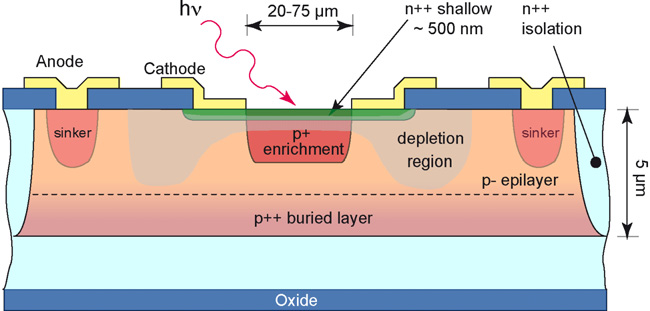
\includegraphics[width=\textwidth]{figure/spad_pixel_struct.jpg}
  \bicaption{Device structure of SPAD.}{SPAD的器件结构。}
  \label{fig:spad_pixel}
\end{figure}

单光子雪崩二极管(SPAD)是一种类似于光电二极管的半导体器件,但具有较大的偏置电压,这会导致载流子倍增:单光子的吸收会导致雪崩击穿,从而产生可由外部电子设备检测和处理的大电流信号,其器件结构如图\ref{fig:spad_pixel}所示\citep{zappa2007principles}。时间-数字转换器测量光子从激光器发射和最后被SPAD检测到之间的时间,然后使用时变单光子计数器形成光子到达时间的直方图\citep{becker2005advanced}。SPAD实现了高单光子灵敏度,其光子探测效率高达40\%,在可见光谱中暗计数率极低,为每秒1-10个光子。在检测到光子后,探测器在数十到数百纳秒的延迟期(死区时间)内无法继续检测光子,因此限制了可实现的最大计数率。
只要测量是在光子稀疏的情况下进行的,也就是说,在死区时间(称为堆积)期间,一个以上光子撞击探测器的可能性基本上小于一个,光子到达时间的直方图给出了光脉冲时间剖面的精确测量。考虑到SPAD死区时间,SPAD在光子稀疏区域工作时,其可提供的最大计数率约为1-10 MHz,以避免光子堆积失真效应。

\begin{figure}[!tb]
  \centering
  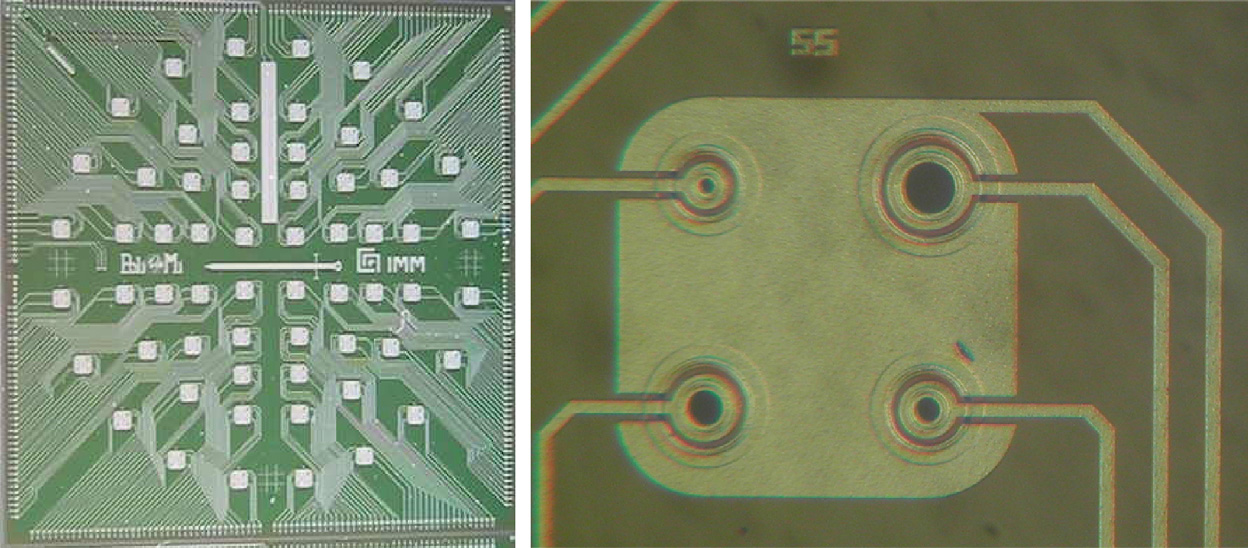
\includegraphics[width=\textwidth]{figure/spad_array.jpg}
  \bicaption{SPAD array的显微照片。左边为18mm$\times$18nm的SPAD array,右边是阵列中的一个4$\times$4的SPAD像素单元。图片来自\citet{zappa2007principles}。}{Microphotograph of an example of the SPAD array. In the left is a 18 $\times$18 SPAD array while in the right is a 4$\times$4 SPAD pixels unit in the array. Picture from \citet{zappa2007principles}.}
  \label{fig:spad_array}
\end{figure}

SPAD传感器有单像素和阵列(即相机)两种形式,既有支持可见光波长的\citep{richardson200932,richardson2011scaleable,gersbach2012time,bronzi2014100,burri2016linospad},也有支持红外波长的\citep{itzler2008geiger,itzler2008single,itzler2007single}。SPAD相机已用于瞬态成像,其单光子灵敏度使其能够捕捉在自由空间传播的光脉冲。相机上收集的光子来自空气中的瑞利散射,而不是表面散射或扩散介质中的增强散射\citep{gariepy2015single}。一个32$\times$32像素SPAD相机的时间分辨率约为50 ps,相当于每秒2亿帧。虽然没有上面讨论的一些技术的速度快(每秒超过1万亿帧),但这个帧速率仍然足以捕捉运动中的光,成像模糊度仅为1.5厘米。这种时间分辨率的微小损失有以下几个好处。首先,相机结构紧凑,使用简单(可以基于标准CMOS技术制造,可在市场上买到,体积小到可以集成到智能手机中);其次,其数据采集速率高,根据现有实验证明,NLOS数据采集过程可以缩短到亚秒级时间尺度\citep{musarra2019non};并且,使用特定激光照明波长的干涉滤光片,也可以在室外和日光条件下使用\citep{Otoole2018,chan2017non}。也有研究者使用SPAD实现了实时的NLOS数据采集\citep{lindell2018towards}。

在首次以SPAD阵列作为成像设备的非视域成像演示中,SPAD相机仅仅以一种简化的配置方式来使用,因此成像系统也只能恢复出隐藏物体的位置,而无法重构物体完整的3D形状\citep{chan2017non}。这种简化使得NLOS成像可以处理动态的隐藏场景。无论是在小规模的实验室设置中,还是在更大规模的角落(距离探测器超过50米)上检测人\citep{gariepy2016detection},对移动目标的数据采集和处理时间都在1秒左右。单像素选通SPAD\citep{buttafava2015non}和带有扫描激光光斑的SPAD线阵列\citep{o2017reconstructing}也可以用于重构完整的3D场景,目前是NLOS成像的一些首选方法,过去几年中,大多数设置使用单像素或阵列格式的SPAD。本文将要着重讨论的基于RSD的NLOS成像系统,其所使用的传感器也是SPAD阵列,如图\ref{fig:spad_nlos_sys_img}所示。

\begin{figure}[!tb]
  \centering
  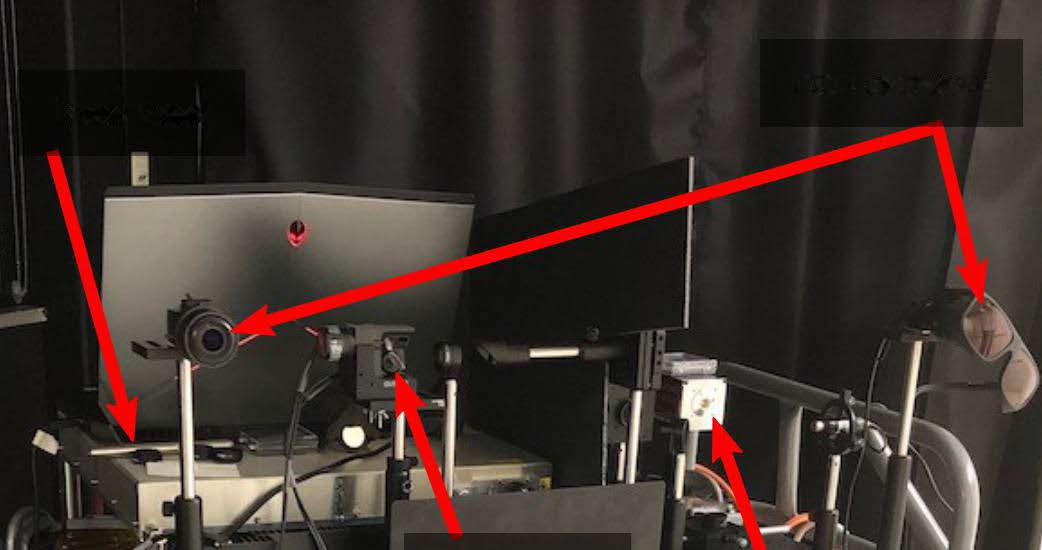
\includegraphics[width=\textwidth]{figure/spad_nlos_sys.pdf}
  \bicaption{\citet{Liu2019}所演示的基于RSD重构算法的NLOS成像硬件系统的照片。}{Photo of the RSD based NLOS imaging hardware system, demonstrated by \citet{Liu2019}.}
  \label{fig:spad_nlos_sys_img}
\end{figure}

目前,大多数SPAD阵列都是为激光雷达成像(LiDAR)而开发的。展望未来,NLOS成像系统需要改进时间分辨率、更好的填充因子、从中继表面阻挡直射光的能力,以及从看到光子的SPAD像素读取光子时间戳的更灵活的方法。因此,我们未来需要为NLOS成像设计专门的SPAD阵列。

\section{非视域成像算法}\label{sec:img_algo}

\subsection{成像模型}

时间分辨探测器如SPAD可以测量在某个时间戳的入射光子通量,其中时间戳代表相对于从脉冲激光器出射光子开始的一个特定时间点。因此,这类探测器可以记录可视区域上,对应于一个时间戳$\tau$,位于$(x',y')$的采样点的时间脉冲响应。对于一个特定的时间戳$\tau$,所有可能的采样点的测量到的脉冲响应组成了一幅瞬时图像(transient image)。而所有的时间戳对应的瞬时图像则组成一个3D时空图像。
如上所述,瞬态图像所测量的既包含来自直接反射的光子通量,也包含沿间接光路径传播的光子通量。前者(即光源发出并从物体散射回探测器的光)包含恢复场景可见部分的形状和反射率所需的所有信息,因此3D成像和激光雷达成像通常使用此类信息来恢复3D场景。而因为它不包含隐藏场景的有用信息,NLOS成像通常不考虑这类来自可视场景直接反射的信息。
通常来说,经过多个表面反射回来的沿间接光路径传播的光子,其到达探测器的时间小于直接反射回来的光子。因此,成像系统利用这一点,即可很容易地移除这些信息。

共焦(confocal)NLOS成像系统的间接光传输的成像模型(即,激光照明和后续检测均位于反射墙上的同一点$(x',y')$)可表述为:
\begin{equation}\label{eq:img_model}
  \begin{split}
    \tau(x',&y',t)=\iiint_\Omega \frac{1}{r^4}\rho(x,y,z)g(x',y',x,y,z)\\ &\delta\left(2\sqrt{(x'-x)^2(y'-y)^2+z^2-tc}\right)\text{d}x\text{d}y\text{d}z,
  \end{split}
\end{equation}
其中$\rho$时隐藏场景中点$(x,y,z)$的反射率;狄拉克函数$\delta$则将光子传播时间$t$和光子第二次反射传播距离$r=\sqrt{(x'-x)^2+(y'-y)^2+z^2}=tc/2$联系起来;$c$是光速;这里我们假设反射墙上所有点$z=0$,且只考虑仅仅经过三次反射的光子;函数$g$则表示了不含时的衰减函数,其仅仅和隐藏物体表面法线、反射率、可见程度等其他因素相关。当成像系统以共焦配置,每测量一次瞬时图像$\tau$,都相当于在隐藏场景的一个球面上做了一次积分(见式\ref{eq:img_model})。

对于更普遍的非共焦(non-confocal)配置方式,激光脉冲器在反射墙面上照明的点和探测器所采样的点不是同一个点。这种配置方式,使得照明点和采样点可以独自扫描,而对应的积分面则是一个椭球面。

NLOS成像模型是绝大多数NLOS成像算法的核心基础,指导着算法从测得的一系列瞬时图像$\tau$中恢复出隐藏物体$\rho$。模型\ref{eq:img_model}中引入的$g$表明所使用的NLOS成像模型是否一个线性的成像模型。有一些简化的NLOS成像算法基于一个线性的NLOS成像模型,即假设$g=1$。这些算法将NLOS成像问题简化为了求解或者近似获得一个线性系统$\mathbf{\tau=A\rho}$的解,其中$\mathbf{\tau}$表示离散化的瞬时图像,$\mathbf{\rho}$表示未知物体的反射率,而$\mathbf{A}$表示一个时间分辨的间接光传输矩阵。这种NLOS成像模型的线性近似,虽然使得重构隐藏物体相比于非线性模型更加简单,但需要对光在隐藏场景的传播作几个前提假设。例如,光线各向同性散射,视线之外的不同场景部分之间不会发生遮挡。实际上,如果模型中包含表面法线、双向反射分布函数和遮挡,视线成像问题也会以类似的方式变得非线性。

除了基于线性NLOS成像模型的算法以外,也有适用于线性和非线性NLOS成像模型的算法。下面一节,本文将介绍几种不同类型的NLOS成像算法。

\subsection{重构算法}

\subsubsection{启发式算法}

用于估计隐藏物体的形状和反射率的启发式重构算法很流行。这些方法中最直观的一种是将第一次返回的间接光子的测量时间与隐藏对象或场景的凸包相关联\citep{Tsai2017},或者,可以拟合简单的参数化平面模型来表示隐藏场景\citep{Pediredla2017}。另一个尚处于起步阶段的领域是使用主动探测方法,该方法根据场景的预期内容塑造照明和检测,以优化探测。第一个散射表面之后的空间重新聚焦可以使用空间光调制器进行控制,聚焦光斑可以在整个场景中进行扫描\citep{starshynov2019coherent}。时间聚焦使用在空间和时间上成形的照明脉冲,在隐藏场景的某个区域创建照明脉冲\citep{pediredla2019snlos}。这些技术可以提高重构算法的信噪比和分辨率。

\subsubsection{反投影算法}

反投影算法是NLOS成像算法中最常用的一类算法。这一类算法将隐藏的场景$\rho$用$\mathbf{A}^T\mathbf{\tau}$来进行估计,并对这一估计的结果做一些如滤波等后处理来获得最终的重构结果。这类策略是解决大规模重构问题例如医学成像的标准解决方案。事实上,共焦NLOS扫描方法的反问题与球面Radon变换密切相关\citep{tasinkevych2014circular},而一般的非共焦扫描方法与椭圆Radon变换类似\citep{moon2014determination}。这些和Radon变换相关的滤波反投影算法的计算时间和存储需求,即使对于那些大规模的重构问题,也是相对容易处理的。因此也有不少基于滤波反投影算法的NLOS成像算法也被研究出来\citep{Velten2012,gupta2012reconstruction,buttafava2014time,Laurenzis2014,Arellano2017}。不过这些成像算法的复杂度普遍较高,对于重构含有$N$个体素的场景,其复杂度为$O(N^5)$。

\subsubsection{线性逆向算法}

线性逆向算法被用来解决由$\tau$估计$\rho$的凸优化问题。其中有几种方法旨在使用迭代优化方法来解决这个问题\citep{gupta2012reconstruction,wu2012frequency,heide2014diffuse},但这些算法性能不好,实际运行太慢。光锥变换\citep{Otoole2018}是线性逆问题的一种闭式解,它通过在待重构物体上假设一个光滑的先验条件,有效地解决了计算复杂度为$O(N^3logN)$的精确线性逆问题。当使用图形处理单元(graphics processing unit, GPU)来实现光锥变换算法时,可以勉强实现实时NLOS重构(大约5 FPS)\citep{DBLP:journals/corr/abs-2010-12737}。

\subsubsection{波动光学算法}

与上述基于几何光学的成像算法相反,基于波动光学的算法最近已被用于使用时间分辨探测器和脉冲光源的瞬态成像配置的NLOS成像系统\citep{Liu2019,DavidB.Lindell2019,Teichman2019,Elten2019,Dove2019}。在这些方法中,隐藏场景中的光传输过程是使用随时间变化的波动方程或其他物理光学模型建模的。类似的概念也适用于振幅调制连续波光源在傅里叶域捕获的NLOS数据\citep{kadambi2013coded}。

与上面讨论的大多数方法不同,这类算法不一定试图直接解决隐藏几何体的重构问题。相反,瞬态图像被视为虚拟波场,并在时间上向后传播到特定的时间瞬间。然后,几何重构问题就变成了将隐藏几何体与时间演化波场的特定特性联系起来的问题。与视域成像相机中一样,该问题被分为估计隐藏场景(即图像)中的波的线性算子和估计图像的几何和双向反射分布函数等特性的非线性问题。

对于NLOS成像问题,波动光学模型有几个好处。
首先,实验证明,其中一些方法对隐藏表面的不同类型的反射特性更具鲁棒性。
光泽、镜面反射、漫反射或回归反射材料都可以用相同的方法处理,而几何光学方法必须事先知道并建模反射特性,或者与隐藏的几何一起估计它们。
其次,波动光学模型使NLOS成像与雷达、地震成像、超声波成像和其他既定领域的相关工作之间的联系变得更加容易。例如,距离偏移技术,包括频率-波数或f-k偏移,最初是在地震成像界开发的\citep{stolt1978migration},后来被用于合成孔径声纳\citep{callow2003signal,sheriff1992synthetic}、超声成像\citep{sheriff1992synthetic}和合成孔径雷达\citep{sheriff1992synthetic},产生了一些最快、最稳健的NLOS成像技术\citep{DavidB.Lindell2019}。这些实验中使用的光波的相位信息不需要测量。取而代之的是光载波上强度波的相位和波前。这种波的相位与信号光子的到达时间有关,而与它们的光学相位无关。时间分辨NLOS成像系统通常无法获取光波的相位。间接光传输的飞行时间信息必须用来估计物体的形状,这使得相关的重构问题有所不同。

\subsubsection{机器学习算法}

数据驱动的机器学习方法正在逐渐成为NLOS重构算法的工具。神经网络可以从连续光源和传统相机捕获的稳态数据中重建隐藏场景\citep{tancik2018data,chen2019steady}。然而,NLOS成像的实际应用中使用机器学习方法会面临一个困难,即如何获得足够的训练数据。一种办法是生成仿真的数据作为训练集,这些数据通过一个已知的光传播模型,渲染一个模拟场景来获得。

\section{研究意义}

回到本文在\ref{sec:backgd}节中提到的NLOS成像技术目前存在的三大挑战,本文\ref{sec:img_sys}节介绍的各类新兴的成像系统基本克服了第一个挑战,使得高精度NLOS成像系统可以在实验室部署。本文\ref{sec:img_algo}节介绍的各类更高效的成像算法则在第二个挑战上取得重大突破,尤其最近两年在快速NLOS成像算法上的突破使得实时NLOS成像成为可能。

第三个挑战近年来也有不少研究工作探索出时间复杂度和空间复杂度上更优化的算法,然而由于NLOS成像问题其在本质上的复杂性,导致其成像算法在通用计算机上的性能仍然无法满足实时成像的速率。表\ref{tab:algo_perf_comp}对比了本文前述的几个快速的NLOS成像算法的重构所需时间以及运行速度。如前文所述,即使GPU加速目前最高效的NLOS成像算法之一的LCT算法,其所能达到的速率也仅仅5 FPS,距离肉眼无法分辨的视频帧率(约24 FPS\citep{read2000restoration})还很远。因此,实现实时NLOS成像还需要进一步的研究。

\begin{table*}[!tb]
    \centering
    \caption{NLOS重构算法性能比较}
    \label{tab:algo_perf_comp}
    \resizebox{\textwidth}{!}{
    \begin{tabular}{@{}cccccc@{}}
    \toprule
    算法     & 重构时间 (s) & 分辨率            & 速度 (voxel/s) & 硬件平台            & 数据采集方式            \\ \midrule
    FBP \citep{Velten2012}           & 1873.34                 & $162\times 162\times 162$ & 2269.9           & i7 CPU              & 非共焦            \\
    Fast FBP \citep{Arellano2017}      & 19.37                   & $162\times 162\times 162$ & $2.15\times 10^5$           & GTX 1060            & 非共焦             \\
    LCT \citep{Otoole2018}           & 1                       & $64\times 64\times 512$   & $2.1\times 10^6$            & i7 CPU              & 共焦                 \\
    LCT \citep{Otoole2018}           & 0.2                     & $64\times 64\times 512$   & $1.05\times 10^7$           & GPU                 & 共焦                 \\
    FK Migration \citep{DavidB.Lindell2019}  & 80                      & $512\times 512\times 512$ & $1.6\times 10^6$            & Xeon E5-2690 v4 CPU & 共焦                 \\
    原始的RSD \citep{Liu}  & 2.4   & $128\times 128\times 69$  & $4.7\times 10^5$            & R7 4800HS CPU   & 非共焦 \& 共焦 \\
    优化的RSD & 0.8   & $128\times 128\times 69$  & $1.41\times 10^6$           & R7 4800HS CPU   & 非共焦 \& 共焦 \\
    优化的RSD & \textbf{0.04}  & $128\times 128\times 69$  & $\mathbf{2.83\times 10^7}$           & Stratix 10 FPGA     & 非共焦 \& 共焦 \\ \bottomrule
    \end{tabular}}
\end{table*}

本文提出一种基于现场可编程门阵列(FPGA)的,专用于加速NLOS成像算法的电路架构,能够在较低的时钟频率(50 MHz)前提下,以25 FPS的帧率重构场景,实现分辨率为128$\times$128的实时NLOS成像。为了能够将算法实现在资源有限的FPGA平台上,本文使用了两种对原算法的优化技术,使得算法的复杂度进一步降低,并充分利用FPGA定制数据流的特点来提高成像算法的吞吐率。截止到目前尚未有研究者使用FPGA或者专用领域集成电路(ASIC)的形式来加速NLOS成像,我们希望本文的研究工作可以作为未来相关工作的一个起点。

\section{内容编排}

本文的内容将按照如下方式进行编排:第一章为绪论部分,简要介绍了非视域成像的研究背景及研究意义,并概述了国内外对于非视域成像领域的相关研究,其中主要包括传感器以及成像算法的两个方面。第二章本文将主要介绍基于瑞利索末菲衍射(RSD)的非视域成像重构算法,包括原始的算法以及针对硬件设计而做的算法优化的两种技巧。第三章进一步分析优化后的基于RSD的非视域成像重构算法的结构和流程,研究针对它的硬件设计可能性,并探索硬件设计空间。第四章基于算法的分析和设计空间探索的结果,详细介绍了NLOS成像加速电路的微架构设计,包括整个算法加速系统以及下面的各个子模块设计。第五章展示了加速电路的微架构在FPGA上实现的结果,也包括优化后的成像算法和原算法的比较。第六章是对本文的工作的总结以及对未来的展望。

\chapter{基于RSD的成像重构算法}
 
基于RSD的NLOS重构算法使用RSD积分来近似光的传播,对共焦和非共焦的NLOS数据均适用\citep{Elten2019}。

\section{基于RSD的重构算法原理}\label{sec:rsd_recons_pp}

\subsection{相量场衍射方法}

我们首先回顾前面所提到的NLOS成像系统采集信号的过程。对于非共焦的情况,如图\ref{fig:rsd_nlos_scene}所示,激光器点亮反射墙上点$P$,并收集从场景反射回反射墙上点$C$的光。采集的数据$H(\mathbf{x_p}\rightarrow \mathbf{x_c},t)$实际上代表了隐藏场景对应的脉冲响应。作为输入信号的$\mathcal{P}(\mathbf{x_p},t)$代表了激光脉冲在反射墙上对应的相量场的波前(phasor field wavefront),我们利用脉冲响应$H(\mathbf{x_p}\rightarrow \mathbf{x_c},t)$可以如下计算经由场景反射到反射墙上的相量场波前
\begin{equation}\label{eq:convt}
  \mathcal{P}(\mathbf{x_c},t) = \int_P \left[ \mathcal{P}(\mathbf{x_p},t) *_t H(\mathbf{x_p}\rightarrow \mathbf{x_c},t) \right] \text{d}\mathbf{x_p}.
\end{equation}
其中,符号$*_t$代表在时域上的卷积,积分则是对整个反射墙所有可能的$\mathbf{x_p}$上进行。

\begin{figure}[!tb]
  \centering
  \includegraphics[width=\textwidth]{figure/relaywall.pdf}
  \bicaption{基于RSD的相量场方法重构隐藏物体。}{Reconstruct hidden objects using RSD based phasor field method.}
  \label{fig:rsd_nlos_scene}
\end{figure}

如何从$\mathcal{P}(\mathbf{x_c},t)$中重构出一个场景,实际上是LOS成像形成的基本问题。这种重构过程可以表达为
\begin{equation}\label{eq:recons}
  I(\mathbf{x_v}, t)=\varPhi (\mathcal{P}(\mathbf{x_c},t)).
\end{equation}
重构算子$\varPhi$相当于将墙上点$C$处的波前反向传播至场景中的点$\mathbf{x_v}$,这些点之中就包括了场景中物体的形状信息。根据相关理论\citep{Teichman2019},频域下的重构算子$\varPhi$作用在相量场波前上可以用RSD积分算符$\mathcal{R}_{\mathbf{x_v}}$来表示
\begin{equation}\label{eq:recons_freq}
  \varPhi \left( \mathcal{P}_F(\mathbf{x_c},\omega) \right) = \Big| \mathcal{R}_{\mathbf{x_v}} \left( \mathcal{P}_F(\mathbf{x_c},\omega) \right) \Big|^2.
\end{equation}
其中,$\mathcal{P}_F(\mathbf{x_c},\omega)$是波前的频域形式。
RSD积分算符的数学形式为
\begin{equation}\label{eq:rsdint}
  \mathcal{R}_{\mathbf{x_v}} \left( \mathcal{P}_F(\mathbf{x_c},\omega) \right) = \alpha(\mathbf{x_v}) \int_C \mathcal{P}_F(\mathbf{x_c},\omega) \frac{e^{-ik|\mathbf{x_c}-\mathbf{x_v}|}}{|\mathbf{x_c}-\mathbf{x_v}|}\text{d} \mathbf{x_c} .
\end{equation}
其中,$k=\omega/c$为波数,单独的小写字母$c$为光速。式子中的$\frac{e^{-ik\mathbf{x_c}-\mathbf{x_v}|}}{|\mathbf{x_c}-\mathbf{x_v}|}$称为RSD核。与传统的RSD积分所不同的是,相量场中的RSD积分引入了一个幅度校正因子$\alpha(\mathbf{x_v})$。它只和场景中的点$\mathbf{x_v}$有关,只要隐藏区域中的物体的反射表面形状已知,它的值就是确定的。由于该因子的仅仅影响重构图像的亮度,而不会改变物体在重构结果中的形状,因此这一项因子往往可以忽略。至此可以形象地说,RSD积分相当于将抵达到反射面C的光波(相量场波前)反向传播回隐藏的场景去,从而重构这个场景。也可以等价的把这一过程认为,存在一个位于反射墙背后的虚拟相机,反射面C则相当于它的相机孔,它根据射到相机孔上的光来重构隐藏场景。

激光脉冲在反射墙的相量场波前的数学模型是已知的,其数学形式为
\begin{equation}\label{eq:impul}
 \mathcal{P}(\mathbf{x_p},t) = e^{i\omega_0 t}\delta(\mathbf{x_p}-\mathbf{x_{ls}})e^{-\frac{(t-t_0)^2}{2\sigma^2}},
\end{equation}
表示在一个虚拟光源(即激光所照亮的点)$x_{ls}$处的波前,其中$\omega_0$表示脉冲的中心频率,决定了激光的波长。中心频率的选择取决于场景中反射墙上的空间采样率。根据采样定理,激光的波长必须大于相邻的$P$、$C$两点之间最大距离的两倍。同时,波长还要大于成像设备的时间分辨率\citep{Liu2019}。比如,给定一个最小的空间采样间隔是1cm,那么波长必须大于2cm。为了方便,表示衰减项的$e^{-\frac{(t-t_0)^2}{2\sigma^2}}$中的$t_0$我们设定为0。
我们进一步将激光脉冲时域模型转换到其对应的频域形式
\begin{equation} \label{eq:impul_freq}
 \mathcal{P}_F(\mathbf{x_p},\omega) = \delta(\mathbf{x_p}-\mathbf{x_{ls}})\cdot \left[ 2\pi\delta(\omega-\omega_0)*_\omega\sigma\sqrt{2\pi}e^{-\frac{\sigma^2\omega^2}{2}} \right].
\end{equation}
其中,符号$*_\omega$同样地表示在$\omega$上做卷积。脉冲模型的频域形式是一个以中心频率$\omega_0$为均值的高斯函数。

对方程(\ref{eq:convt})两边做时域上的的傅里叶变换,得到
\begin{equation}
  \mathcal{P}_F(\mathbf{x_c},\omega) = \int_P \mathcal{P}_F(\mathbf{x_p},\omega) H(\mathbf{x_p}\rightarrow \mathbf{x_c},\omega) \text{d}\mathbf{x_p}.
\end{equation}
由于实际上激光器只会在墙上照亮一个点,因此这里的积分实际上可以省去,得到
\begin{equation}\label{eq:input_trans}
  \mathcal{P}_F(\mathbf{x_c},\omega) = \mathcal{P}_F(\mathbf{x_p},\omega) H(\mathbf{x_p}\rightarrow \mathbf{x_c},\omega).
\end{equation}
这实际上就是SPAD接收到的输入瞬态图像的频域。进一步,
我们将方程(\ref{eq:recons_freq})代入式(\ref{eq:recons})并作傅里叶逆变换得到
\begin{equation}\label{eq:rsd_recons_pp}
  I(\mathbf{x_v},t)=\frac{1}{2\pi}\int_{-\infty}^{+\infty}e^{i\omega t}\Big| \mathcal{R}_{\mathbf{x_v}} \left( \mathcal{P}_F(\mathbf{x_c},\omega) \right) \Big|^2 \text{d}\omega.
\end{equation}
如此,我们便推导出了基于RSD的NLOS重构算法的基本原理。接下来,本文将讨论如何离散化RSD积分$\mathcal{R}_{\mathbf{x_v}}$,并给出快速计算RSD积分的算法。

\subsection{RSD空间卷积方法}

如前所述,RSD将光从反射面反向传播回被重构场景的任一点$x_v$。为便于计算,我们约束光在两个平行的平面上传播,即反射面的点$\mathbf{x_c}=(x_c,y_c,0)$,以及物体上的点$\mathbf{x_v}=(x_v,y_v,z_v)$。将引入的坐标$\mathbf{x_c}$和$\mathbf{x_v}$代入RSD的定义(\ref{eq:rsdint})并省略$\alpha(\mathbf{x_v})$
\begin{equation}\label{eq:rsdconv}
  \begin{split}
    &\mathcal{P}_F(\mathbf{x_v},\omega) = \mathcal{R}_{\mathbf{x_v}}\left( \mathcal{P}_F(\mathbf{x_c},\omega) \right) \\
    &\mathcal{P}_F(x_v,y_v,z_v,\omega) = \mathcal{R}_{z_v}\left( \mathcal{P}_F(x_c,y_c,0,\omega) \right)\\
    &= \iint_{\mathbb{R}^2}\mathcal{P}_F(x_c,y_c,0,\omega)\frac{e^{-i\frac{\omega}{c}\sqrt{(x_c-x_v)^2+(y_c-y_v)^2+z_v^2}}}{\sqrt{(x_c-x_v)^2+(y_c-y_v)^2+z_v^2}} \text{d}x_c\text{d}y_c \\
    &= \iint_{\mathbb{R}^2}\mathcal{P}_F(x_c,y_c,0,\omega) G(x_v-x_c,y_v-y_c,z_v,\omega) \text{d}x_c\text{d}y_c \\
    &= \mathcal{P}_F(x_c,y_c,0,\omega) \circledast G(x_v,y_v,z_v,\omega),
  \end{split}
\end{equation}
其中,我们定义RSD卷积核
\begin{equation}
  G(x,y,z,\omega) = \frac{e^{-i\frac{\omega}{c}\sqrt{x^2+y^2+z^2}}}{\sqrt{x^2+y^2+z^2}}
\end{equation}
而符号$\circledast$表示平面上的二维卷积操作。RSD算符由$\mathcal{R}_{\mathbf{x_v}}$转变下标为$\mathcal{R}_{z_v}$表示这一传播不在仅仅针对一个点$\mathbf{x_v}$而是对平面$z=z_v$上的所有点。对于一个特定的频率$\omega$,反射面C上的相量场波前$\mathcal{P}_F(x_c,y_c,0,\omega)$与相同频率的,深度在$z_v$的RSD卷积核做二维卷积,即可得到传播后的平面$z=z_v$上的相量场波前$\mathcal{P}_F(x_v,y_v,z_v,\omega)$。值得注意的是,这里所提到二维空间卷积和图像处理领域中常见的二维卷积计算方式完全不同,这里所用的“卷积核”概念也和近年流行的卷积神经网络中的卷积核不同,因此利用快速傅里叶变换(FFT)来做快速卷积以优化二维空间卷积的性能是可能的。

%TODO 补图,解释一下二维空间卷积的做法,和卷积神经网络的卷积的不同。

RSD的二维空间卷积需要对所有特定的频率$\omega$进行。考虑到激光脉冲的频率形式(\ref{eq:impul}),波前$\mathcal{P}_F(x_c,y_c,0,\omega)$是一个宽带信号,其频谱是一个以$\omega_0$为中心频率的高斯函数(\ref{eq:impul_freq})。因此,我们考虑一个特定的频率区间$[\omega_0-\Delta \omega, \omega_0+\Delta \omega]$内的几个特定的采样频率即可。所选择的频率范围$2\Delta\omega$主要取决于激光脉冲的带宽,也就是式(\ref{eq:impul})中的脉宽系数$\sigma$。对式(\ref{eq:rsdconv})做在频域上傅里叶逆变换,并只考虑上述频率区间内的积分,得到
\begin{equation}\label{eq:recons4d}
  \mathcal{P}(x_v,y_v,z_v,t)=\int_{\omega_0-\Delta \omega}^{\omega_0+\Delta \omega} e^{j\omega t}\cdot \mathcal{R}_{z_v}\left( \mathcal{P}_F(x_c,y_c,0,\omega) \right) \frac{\text{d}\omega}{2\pi} .
\end{equation}
如此就等价于发送一个设计好的调制脉冲波前
\begin{equation}
  \mathcal{P}(\mathbf{x_p},t)=e^{i\omega_0 t}e^{-\frac{t^2}{2\sigma^2}}
\end{equation} 
到隐藏场景内,随后在可见的反射墙上捕捉到反射回来的波前,并将之传播回到场景中。若把反射墙视作一个虚拟相机孔,这一过程相当于用一个虚拟透镜将场景在一个虚拟图像传感器上成像。式(\ref{eq:recons4d})左边即传播回场景中的波前,是一个关于时间的函数,这是因为场景中每个点都实际上只被脉冲照亮一小段时间。这一函数的绝对值的平方就是我们想要的重构结果。这一结果可以理解为一个三维场景的动态视频,视频内容即隐藏的场景被反射墙上的亮点反射的光,以球面波的方式照亮的过程。

\subsection{时移因子}

然而,我们实际上仅仅关心隐藏场景的形状、物体分布等等,重构一个4D的含时间的场景模型会浪费大量不必要的计算量。真正需要的重构结果,应该仅仅包含场景中的每个点在其刚好被脉冲照亮的那一瞬间,每个体素(voxel)的时间被冻结在激光脉冲的峰值刚好抵达它的那一刻。利用球面几何,我们可以知道光从虚拟光源$\mathbf{x_{ls}}=(x_{ls},y_{ls},0)$处抵达$\mathbf{x_v}=(x_v,y_v,z_v)$所需要的时间
\begin{equation}\label{eq:trav_time}
  t := \frac{1}{c}\sqrt{(x_v-x_{ls})^2+(y_v-y_{ls})^2+z_v^2}.
\end{equation}  
只需要把式(\ref{eq:rsd_recons_pp})中的时间$t$替换为上式,即可得到我们真正想要的3D重构结果。从而,3D虚拟相机只能看到从隐藏物体直接反射的光,对应的体素也只在脉冲刚好抵达的时刻被重构。重构算法不再包含第四个时间的维度,因此提高了重构的效率。

在上一节中提到,RSD空间卷积是将波前反向传播到与反射强平行的平面,而光从光源处却以球面波的形式传播回去。那么理论上,这就意味着平面$z=z_v$上的每个点或者体素上的波前都有不同的相位。这是由于每个点上光的到达时间不同,如式(\ref{eq:trav_time})所示。从而,在对每个平面上的波前做频域上的傅里叶逆变换时,需要对每个体素乘以一个时移因子。

对每个点都采用不同的时移因子的值,会增加算法的复杂度。为了规避这种复杂计算,我们将RSD重构平面$z=z_v$切割为不同的区域,区域内的点看作具有相等的时移因子,即脉冲峰值抵达这一区域内所有点的时间近似相同。激光脉冲的球面传播过程按相同时间段分片,每一段时间内光的传播近似为一个球壳,而整个隐藏场景因此被划分为一系列的具有相同厚度的球壳。球壳与重构平面所交叠的区域内的点近似为具有相同的时移因子。这个空间的切分如图\ref{fig:shell_sect}所示。
\begin{figure}[!tb]
  \centering
  \includegraphics[width=\textwidth]{figure/shell_section.pdf}
  \bicaption{确定时移因子的空间切分。}{Spatial sectioning for determining the peice-wise time shift.}
  \label{fig:shell_sect}
\end{figure}  
图中的$D$表示对应一段时间传播的球壳的厚度,它的取值和激光脉冲的脉宽参数$\sigma$有关。这里我们定义
\begin{equation}
  D = c\cdot \frac{\sigma}{0.15} .
\end{equation}
重构平面上的点$(x_v,y_v,z_v)$所处的区域由其坐标决定。图\ref{fig:shell_sect}中的$E(x_v,y_v,z_v)$表示了平面上的点,到与该平面相切的球壳中心线的距离。判断区域的条件用一个二值条件函数$M_l$来表示,而$E$则构成这一判断,如下
\begin{equation}
  \begin{split}
    &M_1(x_v,y_v,z_v) = \begin{cases}
      1,\qquad 0 \leq E(x_v,y_v,z_v) < \frac{D}{2} \\
      0,\qquad \text{else} 
    \end{cases}, \\
    &M_2(x_v,y_v,z_v) = \begin{cases}
      1,\qquad \frac{D}{2} \leq E(x_v,y_v,z_v) < \frac{3D}{2} \\
      0,\qquad \text{else}
    \end{cases}, \\
    \vdots \\
    &M_l(x_v,y_v,z_v) = \begin{cases}
      1,\qquad (l-\frac{3}{2}D) \leq E(x_v,y_v,z_v) < (l-\frac{1}{2})D \\
      0,\qquad \text{else}
    \end{cases}, 
  \end{split}
\end{equation}
$M_l(x_v,y_v,z_v)$用以判断点$(x_v,y_v,z_v)$是否属于第$l$层球壳,若是则为1,不是则为0。而$E(x_v,y_v,z_v)$可以根据图\ref{fig:shell_sect}给出
\begin{equation}
  E(x_v,y_v,z_v) = \sqrt{(x_v-x_{ls})^2+(y_v-y_{ls})^2+z_v^2} - z_v
\end{equation}
图中的红点代表了反射墙上的虚拟光源,其坐标$(x_{ls},y_{ls},0)$可以看作代表了虚拟相机孔。其发出的激光脉冲随时间推移向外传播,每隔一段时间划分出等厚的球壳,如图中的绿色和橙色球壳。球壳的中心线(如图中的黑色实线)表示激光脉冲的中心峰值处,相邻中心线之间的距离也是$D$。球壳与重构平面相交的部分在平面上划分出以黄色和蓝色标识的区域。区域内的点经过近似,不再被看作被球面波照射,而可以视作由传播了特定距离
\begin{equation}
  B_l = \tilde{D} + (l-1) D
\end{equation}
的平面波照射。其中,$\tilde{D}$代表距离校正常数,对于理想的经过完美校正的系统$\tilde{D}=0$,而对实际的设备则取一个大于0的数字。注意到,重构平面里光源越远,平面与一层球壳相交的部分越大。若考虑无限远的平面,激光脉冲的传播就变成了平面波,整个平面都包含在这一无限大的球壳里。此处所选择的球壳的厚度$D$表征了近似的精确程度,越大的$D$越不精确。球壳近似意味着球壳内的点并非总是在最亮的那个瞬间被重构,因此这一近似会给重构结果的亮度造成一定程度的误差,但不会对重构结果中的物体形状有所影响。

利用上述定义的区域条件函数$M_l$和距离函数$B_l$,理论上重构场景内任意一点$\mathbf{x_v}$的时移因子,即需补偿的相位为
\begin{equation}
  \begin{split}\label{eq:timeshift}
    T(x_v,y_v,z_v,\omega) &= \lim_{L\rightarrow \infty} \sum_{l=1}^L T_l(x_v,y_v,z_v,\omega) \\
    &= \lim_{L\rightarrow \infty} \sum_{l=1}^LM_l(x_v,y_v,z_v)\cdot \exp \left( i\frac{\omega}{c} (z_v+B_l) \right).
  \end{split}
\end{equation}
实际情况下,$D$的量级通常在20\textasciitilde30cm之间,因此大多数的小型简单场景下只需有一层球壳($L=1$)即可。对于较大型的室内场景的应用,球壳层数取到$L=2$即可。更大型的场景需要更多的球壳层数,如果划分的层数较少,那么重构结果会产生渐晕效应(vignetting effect)。这一效应会降低成像质量,如同使用了一个过度简化的透镜设计的成像系统一样。

最后,利用式(\ref{eq:timeshift})定义的时移因子,我们给出最后真正的3D重构结果
\begin{equation}\label{eq:algo_pp}
  I(\mathbf{x_v}) =\left\lvert \int_{\omega_0-\Delta\omega}^{\omega_0+\Delta\omega} \sum_{l=1}^L T_l(x_v,y_v,z_v,\omega) \cdot \left(\mathcal{P}_F(x_c,y_c,0,\omega)\circledast G(x_c,y_c,z_v,\omega)\right) \frac{\text{d}\omega}{2\pi} \right\rvert^2.
\end{equation} 
上式(\ref{eq:algo_pp})即基于RSD的NLOS重构算法的数学原理。从中我们可以看到,相比于最近所提出的几种快速NLOS成像算法,如LCT、FK,基于RSD的NLOS重构算法除了拥有更低的运行时间和更少的存储需求外,更重要的优势即在于其并行性。对于不同采样深度$z_v$的重构平面,重构过程互相独立,可以同时执行。若运行平台的存储资源有限,那么即使顺序执行不同采样深度的重构,其所需的中间缓存数据也更少,其存储效率更高。而LCT、FK两种算法则需要执行三维傅里叶变换,因此其无论计算量还是存储需求都要更大。

\subsection{输入瞬态图像的处理}

这里简要介绍如何从SPAD传感器获得所需的输入瞬态图像,以及如何进行预处理环节。式(\ref{eq:input_trans})描述了瞬态图像的生成,其中$\mathcal{P}_F(\mathbf{x_p},\omega)$是激光脉冲的频域模型,以方程(\ref{eq:impul_freq})描述,而$H(\mathbf{x_p}\rightarrow \mathbf{x_c},\omega)$则由SPAD传感器首先采集时域上的信号$H(\mathbf{x_p}\rightarrow \mathbf{x_c},t)$,再做时域上的傅里叶变换得到。

\begin{figure}[!tb]
  \centering
  \includegraphics[width=\textwidth]{figure/FDH.pdf}
  \bicaption{时域的直方图TDH做傅里叶变换得到傅里叶域直方图FDH。}{Obtain FDH by doing Fourier transformation on the TDH.}
  \label{fig:fdh}
\end{figure}

SPAD使用一个时间相关的单光子计数器(Time Correlated Single Photon Counter, TCSPC)来记录激光脉冲发射后到相关的光子返回的时间。计数器只记录在一个测量时段内的所有返回的光子的抵达时间。时段内,每个光子自己对应一个时间戳,$t_0, t_1\dots t_N$。对一个发光点$\mathbf{x_p}$和采样点$\mathbf{x_c}$,都有
\begin{equation}
  H(\mathbf{x_p}\rightarrow \mathbf{x_c},t) = \sum_{n=1}^N \delta(t-t_n).
\end{equation}
上式称为TCSPC的时域直方图(TDH)。时间戳$t_n$是离散的;时间分辨率由NLOS成像采集系统决定,通常在几个到数十个皮秒级。对该直方图在某个特定的频率$\omega$上做傅里叶变换,
\begin{equation}
  \begin{split}
    H_F(\mathbf{x_p}\rightarrow \mathbf{x_c},\omega) &= \int_{-\infty}^{+\infty} \left( \sum_{n=1}^N \delta(t-t_n) \right) e^{-i\omega t} \text{d}t \\
    &= \sum_{n=1}^N e^{-i\omega t_n}
  \end{split}
\end{equation}
得到傅里叶域的直方图(FDH)。整个计算过程如图\ref{fig:fdh}所示,通过将一个测量时段内的所有光子的时间戳$t_n, n=1,\dots,N$,乘以某个特定的采样频率$\omega_n$构成一个相移$e^{-i\omega_n t_n}$,并全部累加,便得到FDH中对应$\omega_n$的bin。实际预处理的时候,可能存在的上千个时间戳并不需要全部存储,每接收到一个时间戳便计算相应的相移,并将之和先前计算的累加结果相加并保存以和下一个时间戳的相移累加。同理,对于其他所有的$\omega$一样,可以并行的计算。

计算好的FDH还需要和激光脉冲的频域形式(\ref{eq:impul_freq}),在每个采样频率$\omega_n$上相乘。如前所述,$\omega_n$是在区间$[\omega_0-\Delta\omega,\omega_0+\Delta\omega]$内选择。区间的确定取决于脉冲频响幅度大小。我们定义$\gamma$为幅度占最大幅度的比例,对于幅度比例$\gamma$小于某个阈值的$\omega$可以认为对重构过程没有贡献可以忽略。本文中选择的阈值为0.01,即对幅度小于峰值的1\%的频率可以直接忽略。由于脉冲的频域响应是一个高斯函数,因此这一被选择的区间是一个关于中心频率对称的区间。至于采样频率的间隔$\omega_{res}$,则由TDH的采样频率$f_{sampling}$(即时间分辨率的倒数)和TDH的bin的总数$N_{bins}$决定
\begin{equation}
  \omega_{res} = 2\pi \frac{f_{sampling}}{N_{bins}}.
\end{equation}

$\Delta\omega$和$\omega_{res}$共同决定了采样频率的总数$N_\Omega$。这几个设计参数主要和NLOS成像具体的应用场景有关。在较大的场景中,不仅仅采样深度的总数$N_D$(即重构平面的个数)会增加,$N_\Omega$也会增加,因此重构算法所需的计算量和存储需求也会增加。

%TODO 补图:把输入的瞬态图像和FDH的联系,这种数据结构给画出来。

\section{原始的RSD重构算法}

原始的基于RSD的NLOS重构算法的基本思想,是将抵达探测器光圈的光反向传播回到隐藏场景,从而将NLOS成像问题转化为LOS成像问题,而后者则可以使用一个基于相量场衍射的RSD空间卷积快速解决\citep{Liu}。关于这些基本思想的各个环节的数学推导在上一节\ref{sec:rsd_recons_pp}中已经详细叙述。

RSD重构算法流程的简要概念如图\ref{fig:ori_algo_concept}所示。
\begin{figure}[!tb]
  \centering
  \includegraphics[width=\textwidth]{figure/ori_algo_concept.pdf}
  \bicaption{基于RSD的NLOS重构算法的基本概念。}{Basic concept of RSD-based NLOS reconstruction.}
  \label{fig:ori_algo_concept}
\end{figure}
令$P(x_c,y_c,t)$为SPAD探测器在时刻$t$时捕捉到的瞬态图像。RSD算法将瞬态图像的傅里叶域
\begin{equation}
  P_F(x_c,y_c,\omega) = \sum_t P(x_c,y_c,t)e^{-j\omega t}
\end{equation}
作为输入。这里,$x_c$和$y_c$为图像中的像素的坐标,$t$则为该图像对应的时间戳,$\omega$属于傅里叶域中所选择的采样频率的集合$\Omega$。

RSD积分定义了一个名为RSD衍射核的四维张量
\begin{equation}\label{eq:kernel}
  G(x_c,y_c,\hat{z},\omega) = \frac{\exp\left[-i2\pi\cdot\hat{z}^2/(\eta^2)\cdot\sqrt{\hat{r}^2/\hat{z}^2+1}\right]}{\sqrt{\hat{r}^2/\hat{z}^2+1}},
\end{equation}
且
\begin{align}
  \hat{r} &= \sqrt{x_c^2+y_c^2}\label{eq:rxy},\\
  \eta^2 &= \frac{\mathbf{c}\hat{z}}{\delta\omega}.
\end{align}
其中,$\hat{z}$属于离散深度集合$D$,$\mathbf{c}$为光速而$\delta$则表示空间采样间隔。

典型的RSD积分的第一步是将$P_F(x_c,y_c,\omega)$和$G(x_c,y_c,\hat{z},\omega)$,在每个特定的$\omega$和$\hat{z}$上做对$(x_c,y_c)$二维空间卷积。这些二维卷积可以在傅里叶域上如下表示
\begin{equation}\label{eq:conv}
  P_F(x_v, y_v, \hat{z}, \omega) = \mathcal{F}^{-1}\left\{\mathcal{F}\left[P_F(x_c, y_c, \omega)\right]\cdot \mathcal{F}\left[G(x_c, y_c, \hat{z}, \omega)\right]\right\}.
\end{equation}
其中,$\mathcal{F}$表示了二维傅里叶变换(FT),$\mathcal{F}^{-1}$表示二维傅里叶逆变换(IFT)。为了得到最终重构的结果,需要对$P_F$在所有采样频率上做一次积分
\begin{equation}
  I(x_v, y_v, \hat{z}) = \sum_{\omega \in  {\Omega}}\sum_{l=1}^{L} T_l(\omega, \hat{z}) P_F(x_v, y_v, \hat{z}, \omega)
\end{equation}
且
\begin{align}
    &T_l(\omega, \hat{z}) = \exp\left[i\frac{\omega}{c}(\hat{z}+B_l)\right],\label{eq:ts} \\
    &B_l =\tilde{\mathbf{D}} + (l-1)\cdot \mathbf{c}\cdot \frac{\sigma}{0.15}.
\end{align}
这里,$T_l$为时移因子,用于补偿光的球形传播导致的相位差,且其中$B_l$表示第$l$个平面所对应的位移;$\tilde{\mathbf{D}}$为校准系数,对于理想系统$\tilde{\mathbf{D}}=0$;$\sigma$表示脉冲宽度。$I(x_v,y_v,\hat{z})$代表了带有场景深度$\hat{z}$的最终三维重构结果,表示隐藏的场景及物体。

\section{优化的RSD重构算法}

尽管相比于现有的NLOS成像算法,RSD重构算法是目前适用于非共焦NLOS数据的最快速的成像算法,其依然存在大量的计算和存储需求。令$N_\Omega$为采样频率集合$\Omega$的势,$N_D$为离散深度集合$D$的势,那么重构一个隐藏的三维场景需要做$N_\Omega\times N_D$次二维卷积。如式(\ref{eq:conv}),每次卷积需要做两次二维傅里叶变换以及一次二维傅里叶反变换,因此重构一次场景所需的傅里叶变换次数(包括反变换)为$3\times N_\Omega \times N_D$。令输入瞬态图像的分辨率为$K\times K$,那么存储所有的RSD核所需的容量为$N_\Omega\times N_D\times K\times K$。另外,为了执行二维卷积,处理器需要大量访问存储单元来获取一个$K\times K$的RSD核。众所周知,对于现代的数字电子系统而言,存储访问耗费大量时间和能量从而往往成为系统的性能瓶颈\citep{hennessy2011computer}。

\begin{figure}[!tb]
    \centering
    \subfloat[]{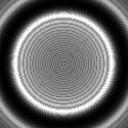
\includegraphics[width=.45\textwidth]{figure/kabs_gray.jpg}} \hspace{10mm} \\
    \subfloat[]{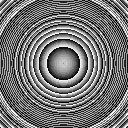
\includegraphics[width=.45\textwidth]{figure/kang_gray.jpg}}
    \bicaption{(a) RSD核幅度图 (b) RSD核相量图。}{(a) The magnitude of an RSD kernel. (b) The phase of an RSD kernel.}
    \label{fig:kernel}
\end{figure}

从式(\ref{eq:kernel})和(\ref{eq:rxy})中可以看出RSD核具有径向对称的特性。如图\ref{fig:kernel},我们也能从RSD核的幅度和相位分布看出这种径向对称的特性。因此,我们可以利用RSD核的这种径向对称性以及傅里叶变换的线性性质,可以显著地减少存储需求以及存储访问次数。图\ref{fig:opt_algo}展示了优化RSD重构算法的基本概念。首先是利用一组RSD核的基函数——半径不同的单位环形脉冲函数——和每个基函数对应的系数,来实时构成傅里叶域的RSD核。同时,如图\ref{fig:opt_algo}(b)通过进一步在径向上采样,基函数可以进一步被一个一维向量重构。最后的结果显示,RSD重构算法执行过程中,总的存储需求以及存储访问次数有了大幅降低。本文将在下面两个小节将详细介绍以上提到上述的两种环形采样和径向采样技术。

\begin{figure}[!tb]
    \centering
    \subfloat[]{\includegraphics[width=\textwidth]{figure/opt_algo.pdf}}\\ \vspace{6pt}
    \subfloat[]{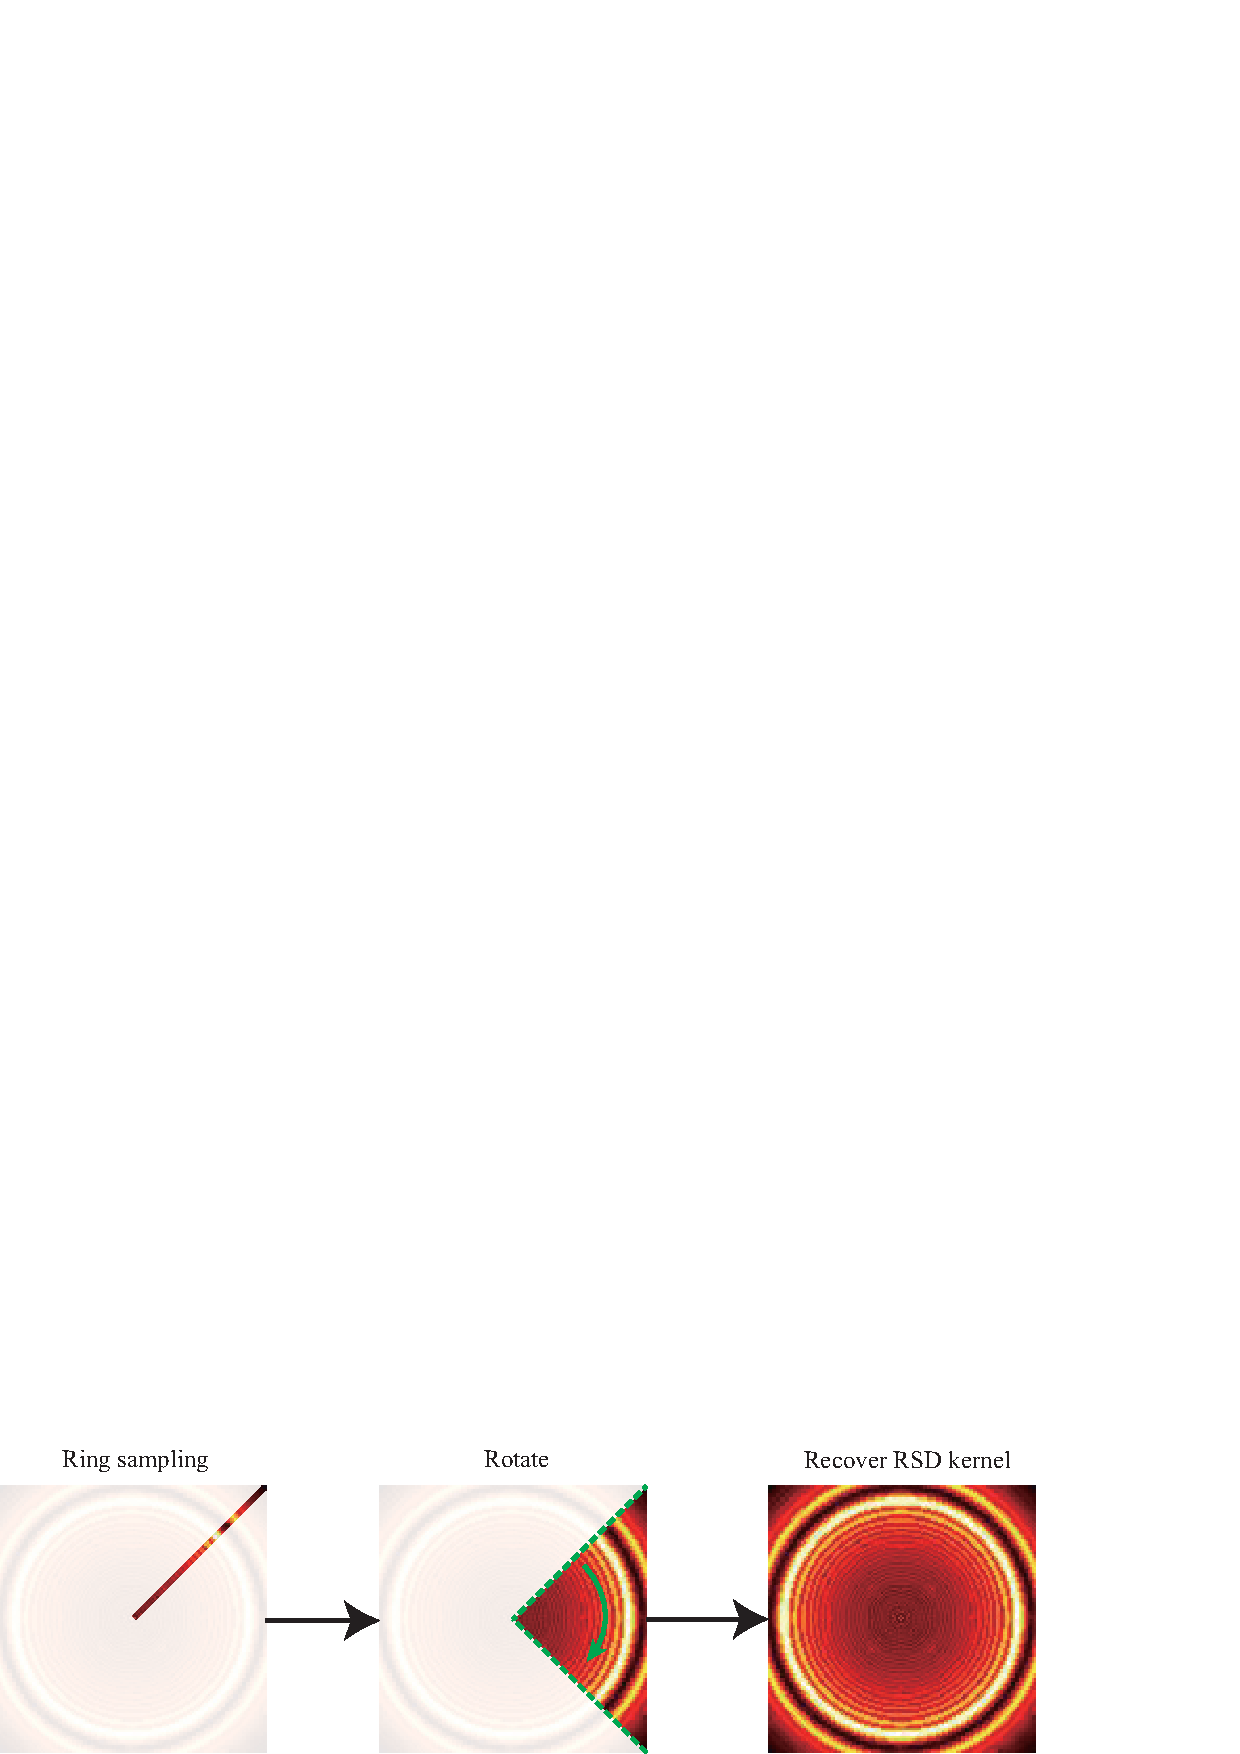
\includegraphics[width=\textwidth]{figure/addrmap1.pdf}}
    \bicaption{优化RSD重构算法的基本概念。 (a) 利用单位环形脉冲和对应的系数来重构RSD核。 (b) 利用地址重映射来重构单位环形脉冲。}{Basic concept of the optimized RSD algorithm. (a) Reconstruction of RSD kernels using unit ring impulses and corresponding coefficients. (b) Reconstruction of unit rings using address mapping.}
    \label{fig:opt_algo}
\end{figure}

\subsection{环形脉冲采样技术}

从图\ref{fig:kernel}中可以看出,RSD核是径向对称的,因此其可以如图\ref{fig:opt_algo}(a)被表达为一组有不同半径长度的单位环形脉冲函数的线性组合
\begin{equation}
    G(x, y, \hat{z}, \omega) = \sum_{i=1}^{N_R}\hat{G}(r_i, \hat{z}, \omega)\delta(x, y, r_i),
\end{equation}
其中,单位环形脉冲函数定义为
\begin{equation}
    \delta(x, y, r_i) = \begin{cases}
      1, & \sqrt{x^2+y^2} = r_i\\
      0, & \sqrt{x^2+y^2} \neq r_i
    \end{cases}\label{eq:ring_imp},
\end{equation}
而对应于不同半径的单位环形脉冲函数的线性组合系数为
\begin{equation} \label{eq:ori_coef}
    \hat{G}(r_i, \hat{z}, \omega) = \frac{\exp{\left[-i2\pi\cdot\hat{z}^2/(\eta^2)\cdot\sqrt{r_i^2/\hat{z}^2+1}\right]}}{\sqrt{r_i^2/\hat{z}^2+1}},
\end{equation}
其中,$r_i$是半径长度集合$R$中的第$i$个单位环形脉冲函数的半径。利用傅里叶变换的线性性质,RSD核的傅里叶频域表示为
\begin{equation}
    \mathcal{F}\left[G(x, y, \hat{z}, \omega)\right] = \sum_{i=1}^{N_{ {R}}}\hat{G}(r_i, \hat{z}, \omega)\mathcal{F}\left[\delta(x, y, r_i)\right],
\end{equation}
其中,$\mathcal{F}$表示针对$xy$平面的二维傅里叶变换。根据式(\ref{eq:ring_imp})定义,单位环形脉冲函数可以由$\delta(x,y,r_i)$重新表示为$\delta(r,r_i)$。对于第$i$个单位环形脉冲函数,其傅里叶频域表达为
\begin{equation}
    \begin{split}
        \delta_{\mathcal{F}}(\rho, r_i)&=\int_0^{+\infty}\left(\int_0^{2\pi}e^{-2\pi r\rho \cos (\theta)}d\theta\right)\delta(r, r_i)rdr\\
        &=\int^{2\pi}_0e^{-2\pi r_i\rho \cos \theta}d\theta \cdot r_i = \mathcal{F}\left[ \delta(r,r_i) \right].
    \end{split}
\end{equation}
注意到,只要单位环形脉冲函数的半径$r_i$确定,其对应的频域$\delta_{\mathcal{F}}(\rho,r_i)$的值就是确定的。利用这一点,我们可以预计算好单位环形脉冲函数的频域的值,并存储起来以省略去这一部分的傅里叶变换的计算,从而大大减少算法运行时所需的计算量。由此,RSD核的频域表示可以通过将每个半径的单位环形脉冲函数的频域表示乘以对应半径的线性系数,并将乘积在半径上进行累加来重构。这样的优化可以使得计算RSD核所需的总存储量以及存储访问量大大减少。

\subsection{径向采样技术}

利用径向对称的函数其二维傅里叶变换后的函数同样也是径向对称的性质\citep{baddour2011two},我们可以仅仅利用频域上的单位环形脉冲函数的径向上的值来重构整个函数。这样我们对于单位环形脉冲函数的存储从原来的二维矩阵缩减到了仅仅半径上的一个一维向量,如图\ref{fig:imp_rad}。
\begin{figure}[!tb]
    \centering
    \includegraphics[width=\textwidth]{figure/imp30.pdf}
    \bicaption{单位环形脉冲函数在半径上的采样。}{Radius sampling of unit ring impulses.}
    \label{fig:imp_rad}
\end{figure}

如图\ref{fig:opt_algo}(b)所示,若要从一个沿半径采样获得的一维向量中重构出完整的二维单位环形脉冲函数的频域,需要一个二维地址映射从一维向量中找到二维单位环形脉冲函数矩阵中每个元素的值。这一地址映射将矩阵元素的笛卡尔坐标转换为相应的用于描述单位环形脉冲函数的极坐标。理论上,这个地址映射不会有任何影响,但由于这一操作在实际运行时是离散的,我们使用的地址映射函数$M(x,y)$定义如下
\begin{align}
    &s=\sqrt{(x-K/2)^2+(y-K/2)^2},  \\
    &\rho = M(x, y) = round\left( s\cdot \frac{N_{\rho}-1}{\frac{\sqrt{2}}{2}K} \right)+1,\label{eq:mapping_func}
\end{align}
其中,$s$是采样点到一个原始的$K\times K$的矩阵中心点的距离,$N_\rho$是半径上采样点的个数。注意到,由于映射函数$M(x,y)$及其操作的对象是离散的,因此利用它来重构RSD核会导致一定程度上的精度损失。图\ref{fig:smp_comp}展示了随着在半径上的采样点个数从10到200的变化,优化后的RSD重构算法所得结果与原始算法结果的相似度变化。这里所用的相似度的测量算法是结构相似度(Structural Similarity,SSIM)。两个图片之间的SSIM值越大表明两者越相似,最大为1时表示两张图片完全相同。从图\ref{fig:smp_comp}中我们可以看到在采样点个数达到了100个以上后,相似度基本持平在0.9左右,而若采样点从100下降到10时,相似度将迅速下降到0.5以下。
\begin{figure}[!tb]
    \centering
    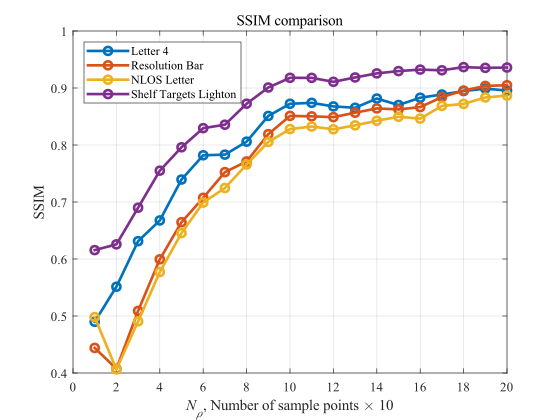
\includegraphics[width=\textwidth]{figure/smp_Nrho_comp_ssim.pdf}
    \bicaption{不同的半径采样点个数下,径向采样的重构结果与原始算法的重构结果的相似度对比。}{Similarity measurement between the radius-sampled results and original results, against different numbers of sampling points $N_{\rho}$.}
    \label{fig:smp_comp}
\end{figure}

同样可以看到这一地址映射操作不仅仅可以用在单位环形脉冲函数上,也可以用在RSD核重构上,即地址映射操作在算法处理流程中的次序不会影响到最终RSD核的重构结果。经过径向采样技术对算法的优化,存储单位环形脉冲函数所需的容量从$K\times K$减少到$\frac{\sqrt{2}}{2}K$。

\subsection{优化后的RSD重构算法}\label{sec:opt_algo}

\begin{table}[!t]
    \centering
    \bicaption{原始算法和优化后算法的复杂度比较}{Complexity Comparison between Original and Optimized RSD Algorithms}
    \label{tab:fuzadu_comp}
    % \resizebox{.98\textwidth}{!}{%
        \begin{tabular}{@{}ccc@{}}
            \toprule
            算法               & 计算量 & 存储访问 \\ \midrule
            原始RSD算法 & $O(N_DN_{\Omega}K^2\log K)$          & $O(N_DN_{\Omega}K^2)$             \\
            优化后的RSD算法& $O(N_DN_{\Omega}K^2)$              & $O(N_{\Omega}K^2)$             \\ \bottomrule
        \end{tabular}%
    % }
\end{table}

经过前述两节介绍的优化技巧,优化后的基于RSD的NLOS重构算法由两部分组成:(i)运行前的算法以及(ii)运行时的算法。前者包括单位环形脉冲函数集和相应的线性组合系数的预计算,可以存储在硬件设备上;后者则是利用预计算的数据和实时采集的NLOS成像数据来重构隐藏场景的成像算法,需要在硬件上实时运行。因此这里作为预计算部分的前者不会实际影响到成像系统的整体性能。这两部分的算法伪代码在算法\ref{algo:b_rt}和算法\ref{algo:rt}中有详细说明。

表格\ref{tab:fuzadu_comp}分别展示了原始算法和优化后算法的RSD算法的计算复杂度和存储访问量。如前面章节所讨论的,原始算法中大量的二维傅里叶变换是其瓶颈所在。因此,重构RSD核所需的计算量和存储量在衡量和比较原始算法和优化后的算法之间的复杂度时必须考虑进去。

\begin{algorithm}[!t]
    \caption{运行前算法}
    \label{algo:b_rt}
    \begin{algorithmic}[1] % The number tells where the line numbering should start
        \Require 采样深度$\hat{z}$; 采样频率$\Omega$; 采样半径$r$。
        \Ensure 预计算数据%\\
        \State 求解输入信号的频率响应:
        \For{$q \gets 1, N_{\Omega}$}
            \State $ P_F(x_c, y_c, \omega_q) \gets \sum_t[P(x_c, y_c, t)e^{-i\omega_q t}] $
        \EndFor
        \State 计算单位环形脉冲函数的傅里叶表示:
        \For{$j \gets 1, N_{R}$}
            \For{$k \gets 1, N_{ {\rho}}$}
                \State $$ \delta_{\mathcal{F}}(\rho_k, r_j) \gets \int_0^{2\pi}r_je^{-2\pi r_j \rho_k \cos \theta} \text{d}\theta $$
            \EndFor
        \EndFor
        \State 计算线性组合系数:
        \For{$q \gets 1, N_{\Omega}$}
            \For{$p \gets 1, N_D$}
                \For{$k \gets 1, N_R$}
                    \State $$\hat{G}(r_k, \hat{z}_p, \omega_q) \gets \frac{\exp{\left[-i2\pi\cdot\hat{z}_p^2/(\eta^2)\cdot\sqrt{r_k^2/\hat{z}_p^2+1}\right]}}{\sqrt{r_k^2/\hat{z}_p^2+1}}$$
                    \State $$ \hat{G}(r_k, \hat{z}_p, \omega_q) \gets \hat{G}(r_k, \hat{z}_p, \omega_q) \cdot \exp\left[i\frac{\omega_q}{c}(\hat{z}_p+B_l)\right] $$
                \EndFor
            \EndFor
        \EndFor
        % \State Generate address mapping matrix 
        % $$
        %     M_{xy} \gets round\left( \frac{\sqrt{(x-K/2)^2+(y-K/2)^2}}{K/2*\sqrt{2}/(N_{ {r}}-1)} \right)+1
        % $$
    \end{algorithmic}
\end{algorithm}

\begin{algorithm*}[!t]
    \caption{Algorithm at runtime}
    \label{algo:rt}
    \begin{algorithmic}[1]
        \Require 瞬态图像$P_F$; 环形脉冲$\delta_{\mathcal{F}}$; 组合系数$\hat{G}$
        \Ensure 重构结果$I$
        \Procedure{Reconstruction}{$P_F, \delta_{\mathcal{F}}, \hat{G}$}
        \For{$i \gets 1, N_{ {D}}$}\Comment{循环1:采样深度上迭代}
            \For{$j \gets 1, N_{ {\Omega}}$}\Comment{循环2: 采样频率上迭代}
                \State $\mathcal{P}_F(x, y, \omega_j) \gets \text{FFT2}(P_F(x, y, \omega_j))$
                \For{$k \gets 1, N_{ {R}}$}\Comment{不同半径上迭代}
                    \For{$l \gets 1, N_{\rho}$}\Comment{所有径向采样点上迭代}
                        \State $G(\rho_l, \hat{z}_i, \omega_j) \gets G(\rho_l, \hat{z}_i, \omega_j) + \hat{G}(r_k, \hat{z}_i, \omega_j)\cdot \delta_{\mathcal{F}}(r, r_k) $
                    \EndFor
                \EndFor
                \For{$x \gets 1, K$} \Comment{在所有坐标上迭代}
                    \For{$y \gets 1, K$}
                        \State $G^{\prime}(x, y, \hat{z}_i, \omega_j) \gets G(M(x, y), \hat{z}_i, \omega_j)$ \Comment{地址映射}
                        \State $ S_F(x, y, \hat{z}_i, \omega_j) \gets \mathcal{P}_F(x, y, \omega_j) \cdot G^{\prime}(x, y, \hat{z}_i, \omega_j) $ 
                    \EndFor
                \EndFor
                \State $I_F(x, y, \hat{z}_i) \gets I_F(x, y, \hat{z}_i) + S_F(x, y, \hat{z}_i, \omega_j)$ \Comment{对所有采样频率累加}
            \EndFor
            \State $I(x, y, \hat{z}_i) \gets \text{IFFT2} \left[ I_F(x, y, \hat{z}_i) \right]$ \EndFor 
        % Do 2D inverse Fourier transformation
        \EndProcedure
    \end{algorithmic}
\end{algorithm*}

\chapter{RSD重构算法加速电路设计}
本章讨论对前述的优化后的基于RSD的NLOS重构算法,包括其任务流程的分析和针对硬件架构设计的进一步优化和取舍。基于对算法的分析,我们使用定量化方法来探索硬件架构的设计空间,以作为后面电路微架构设计的理论基础。

\section{重构算法的分析} 
本章节将对实时NLOS重构算法\ref{algo:rt}进行深入分析,并讨论其引入的一些设计上的挑战以及相应的解决方案。

\subsection{任务流程分析}
运行时NLOS重构算法的流程图如图\ref{fig:tsk_flow}所示。整个算法流程中存在四个计算密集和存储访问密集的任务:
\begin{enumerate}
  \item 由单位环形脉冲函数和线性组合系数重构RSD核。
  \item 对输入瞬态图像的二维傅里叶变换。
  \item RSD核与瞬态图像的频域做的乘累加操作。
  \item 对累加结果的二维傅里叶逆变换。
\end{enumerate}
\begin{figure}[!tb]
    \centering
    \includegraphics[width=\textwidth]{figure/taskflow.pdf}
    \bicaption{运行时重构算法的流程图}{Flowchart of the runtime reconstruction algorithm.}
    \label{fig:tsk_flow}
\end{figure}

整个重构过程可以被分割成$N_D\times N_\Omega$个执行周期。其中每个执行周期用深度计数器和频率计数器的值以$(d,f)$形式标记,因此整个重构过程由执行周期$(0,0)$开始,一直迭代到最后一个执行周期$(N_D-1,N_\Omega-1)$。在以上四个任务中,任务1到任务3在每个执行周期均会被执行,而任务4则只在频率计数器$f$计数至$N_\Omega$时执行。我们可以看到任务1和任务2时相互独立的,因此它们可以被并行执行。而任务3——乘累加任务——则是对任务1和任务2的结果有所依赖。一旦频率计数器计满至$N_\Omega$,任务3乘累加的结果被输入给任务4,以重构相应于深度计数器值的深度的隐藏场景。输入的瞬态图像可以表示为一个多通道的图像,一个$K\times K\times N_\Omega$的张量,单位环形脉冲函数总体表示为一个$N_R\times N_\rho$的矩阵,其线性组合系数则可以表示为一个$N_D\times N_\Omega\times N_R$张量。

对每一个执行周期,二维快速傅里叶变换(FFT)处理器需要读取$K\times K$个像素,并输出其傅里叶变换后的结果。假设瞬态图像的输入通道的传输速率为每个时钟周期传送一个像素,那么一共需要$K\times K\times N_D\times N_\Omega$个时钟周期来读取整个瞬态图像。对于一个典型的NLOS成像系统配置\citep{Liu2020},其中各个参数配置为$K=128, N_D=51, N_\Omega=69$,读取瞬态图像一共需要耗费57655296个时钟周期。我们可以自然地想到一个解决这一问题的想法,即仅仅对所有采样频率点上的瞬态图像做一次二维傅里叶变换,并将其结果存储在本地,随后的执行周期复用这一结果即可。这样一来,好处是可以将读取时间降低至$K\times K\times N_\Omega$个时钟周期,而坏处则是需要更大的片上存储单元来缓存中间结果。

\subsection{线性组合系数分解}

在章节\ref{sec:opt_algo}分析优化后的基于RSD的NLOS重构算法时,我们将线性组合系数的计算放在运行前算法部分,作为与计算的结果存储在本地供运行时算法使用。好处是可以降低运行时的计算负载,但坏处则是引入很大的存储需求。这里,为了进一步降低片上存储单元的使用量,微调了两部分算法的切分,将一部分线性组合系数的计算转移至运行时。注意到,由于傅里叶变换的线性性质,时移因子$T_l$可以被合并至线性组合系数$\hat{G}$里。因此,对应于单位环形脉冲函数的线性组合系数(\ref{eq:ori_coef})可以被重新定义为
\begin{align} \label{eq:coef}
    \hat{G}(r, \hat{z}, \omega) & = \frac{\exp{\left[-i2\pi\cdot\frac{\delta \omega\hat{z}}{\mathbf{c}}\cdot\sqrt{r^2/\hat{z}^2+1}\right]}}{\sqrt{r^2/\hat{z}^2+1}},\\
    \tilde{G}(r, \hat{z}, \omega) & = \hat{G}(r, \hat{z}, \omega) \cdot T_l .
\end{align}
这里,我们引入三个独立的中间变量来进一步分解上述定义的线性组合系数,
\begin{equation}
    W(r, \hat{z}) = \sqrt{\frac{r^2}{\hat{z}^2}+1},
\end{equation}
\begin{equation}
    D(\omega, \hat{z}) = \frac{\delta \omega \hat{z}}{\mathbf{c}},
\end{equation}
\begin{equation}
    T(\omega, \hat{z}) = T_l= \exp \left[ i\frac{\omega}{\mathbf{c}}(\hat{z}+B_l) \right].
\end{equation}
这三个中间变量可以利用选取好的采样深度$\hat{z}$,采样频率$\omega$,以及不同的环形半径$r$来预先计算,并存储为三个可以被深度计数器$d$和频率计数器$f$索引的矩阵。在本文中,我们将这三个变量$W,D,T$分别命名为\textit{wave, distance}和\textit{timeshift}. 而上述重新定义的线性组合系数可以被这三个中间变量重新组合
\begin{equation}
    \tilde{G}(r, \omega, \hat{z}) = \frac{\exp(-i2\pi W(r, \hat{z}) \cdot D(\omega, \hat{z}))}{W(r, \hat{z})} \cdot T(\omega, \hat{z}).
\end{equation}

在运行时,加速器将会在每个执行周期读取$D$和$T$的一个元素,并在频率计数器$f=0$的执行周期,$(0,0),(1,0)$……$(N_D-1,0)$内读取$W$的一列元素。对系数的重新组合过程可以由一些基本的运算部件来承担,如两个乘法器、一个除法器以及一个处理特殊函数
\begin{equation}
    f(t) = e^{-i2\pi t}
\end{equation}
的计算单元。这里的系数分解方法仅仅是为了在设计复杂度、片上存储单元面积大小以及存储访问次数之间取得均衡所做的取舍,同时在不对系统造成性能上的负面影响的前提下尽量提升功耗和面积效率的一种手段。

\section{设计空间探索}\label{sec:dse}

本章节将会引入一些主要的NLOS成像加速器设计参数来定量化的描述设计空间,以探索数据流优化的最佳参数配置。另外,这里还介绍了一个数据复用的方法以跳过一些冗余的计算过程。

这部分关于设计空间探索的讨论目的仅仅是为了尝试不同的架构,并使用对应重构任务的计算时间来衡量其性能。因此,此处仅仅是不包含任何具体微架构实现细节的理论分析。最终的微架构及数据流的设计抉择均基于这部分的分析结果以及架构的硬件可实现性。本文所提出的电路微架构将在下一章中详细讨论。

\subsection{重构延时}

在讨论设计参数之前,我们首先讨论算法按照流程图\ref{fig:tsk_flow}顺序执行时,所占用的运行时间,即任务的总延时。对于章节\ref{sec:opt_algo}所讨论的优化后RSD算法,算法\ref{algo:rt}的延时可以定量化的表达为
\begin{equation} \label{eq:no_opt_lat}
    T_{total} = N_D \{ N_{\Omega}[ \max (T_{FFT}, N_RN_{\rho}T_{ACG}+K^2T_M)+ K^2T_{mul}+T_{ACS} ] + T_{IFFT}\}.
\end{equation}
这里,我们假设FFT模块和RSD核生成模块是相互独立运行的,因此它们可以并行执行。式(\ref{eq:no_opt_lat})中,$T_{FFT}$和$T_{IFFT}$分别表示FFT操作和IFFT操作的延时。通常,FFT模块以每个时钟周期接收一个像素作为输入,因此$T_{FFT}$和$T_{IFFT}$至少需要$K^2$个时钟周期。$T_{ACG}$和$T_{ACS}$则是分别是每次累加$G$和$S_F$所耗费的延时,也就是一个正常的加法器的延时。$T_{mul}$则是乘法的延时和$T_M$则是地址映射操作所需的延时。不失一般性的,我们假设$T_{ACG},T_{ACS},T_{mul},T_M$均为一个时钟周期。

我们考虑一个典型的基于RSD的NLOS重构算法的成像系统\citep{Liu2020},其中各参数配置为$N_D=51, N_\Omega=69, N_R=68, N_\rho=101, K=128$。将这些参数代入式(\ref{eq:no_opt_lat})中可以算出$T_{total}=140318187$时钟周期。这意味着对于一个运行在时钟频率为100MHz的加速器,也需要至少1.4秒才能重构一帧三维隐藏场景,而这样的成像速率无法满足实时NLOS成像的要求。

\subsection{展开因子}

从式(\ref{eq:no_opt_lat})中我们可以看到,算法中的关键路径在于输入瞬态图像做的二维FFT以及RSD核的生成。从算法\ref{algo:rt}中可以看到这部分计算来自于内部循环的迭代。因此若要硬件加速算法的执行,需要从这部分循环的执行开始着手。在此为了定量化描述硬件对算法的加速,我们引入展开因子作为参量,表明循环是如何被展开以使得循环内的操作可以被全部或部分的并行化执行。例如,若有一个需要做$N$次迭代的循环,给它设立一个展开因子$P$,那么这一循环的执行时间减少至$\lceil N/P \rceil$。

对算法\ref{algo:rt}中每个循环,我们都设立一个对应的展开因子,分别为$P_D$, $P_\Omega$, $P_R$, $P_\rho$, $P_x$, $P_y$。那么考虑上这些展开因子后,式(\ref{eq:no_opt_lat})重新写为
\begin{equation}
    \begin{split}
        T_{tot} &= \frac{N_D}{P_D} \Biggl\{ \frac{N_{\Omega}}{P_{\Omega}} \Bigl[ \max (T_{FFT}, \frac{N_{ {R}}N_{\rho}}{P_{ {R}}P_{\rho}} T_{ACG}+\frac{K^2}{P_xP_y}T_M)\\ &+ \frac{K^2}{P_xP_y}T_{mul}+T_{ACS} \Bigr] + T_{IFFT}\Biggr\} \label{eq:opt_lat}.
    \end{split}
\end{equation}

式(\ref{eq:opt_lat})描述了重构任务的总延时和展开因子之间的关系。我们可以说这六个展开因子部分地构成了加速器架构的设计空间。利用式(\ref{eq:opt_lat})我们可以在设计空间中找出一个合适的参数组合,使得对应的重构任务的总延时可以满足特定应用下实时NLOS成像的基本要求。当然,我们可以通过穷尽所有可能的展开因子组合以遍历整个设计空间,但这样做不仅仅耗费大量的时间,而且不适当的展开因子的组合往往导致不规整的架构设计,从而导致复杂的控制结构和数据流,增加了设计的复杂度。循环的展开往往意味着一部分运算部件的复制或流水线的切分,即导致更大的硬件资源或面积消耗。% 后面讲到内部循环的展开往往复制的电路会更小一点,这一句不一定对。

\subsection{数据复用}

对于算法\ref{algo:rt},尽管利用精心组合的展开因子对其进行循环展开是一个关键的优化加速手段,算法中仍然存在一些本身就会耗费大量计算时间的操作需要进一步优化,如FFT和IFFT。不像乘法亦或加法这类代数操作往往最多仅仅需要几个时钟周期即可完成,这类运算模块由于其数据带宽等硬件的限制往往需要上千个时钟周期来完成操作。

算法\ref{algo:rt}中,对输入瞬态图像的二维FFT在循环1和循环2中一共需要迭代$N_D\times N_\Omega$次。然而,可以看到输入的瞬态图像$P_F(x,y,\omega_j)$仅仅和循环2的下标$j$相关而与循环1的下标$i$无关,即其经过二维FFT后的结果对循环1的每次迭代均相同。如果我们缓存这部分结果在片上存储单元并在随后循环1的迭代中复用这部分数据即可大大减少冗余的计算量。因此,重构任务的总延时可以重新描述为
\begin{equation}
    \begin{split}
        &T_{tot} = \frac{N_D}{P_D} \Biggl\{ \frac{N_{\Omega}}{P_{\Omega}} \Bigl[ \frac{N_{ {R}}N_{\rho}}{P_{ {R}}P_{\rho}} T_{ACG}+\frac{K^2}{P_xP_y}T_M \\ &+ \frac{K^2}{P_xP_y}T_{mul}+T_{ACS} \Bigr] + T_{IFFT}\Biggr\} + \frac{N_{\Omega}}{P_{\Omega}} T_{FFT}. \label{eq:tt}
    \end{split}
\end{equation}
这里,我们略微修改了算法的执行过程,以存储中间结果并在之后的执行中进行数据的复用,从而避免了二维FFT的延时。由于循环1的每次迭代所用的FFT的结果都和第一次迭代所用的相同,因此这一复用不会影响算法最后的重构结果。在此基础上,再根据特定的应用场景下实时NLOS成像的要求以及所选择的硬件实现平台的资源限制,选择一个合适的展开因子组合。所选择的展开因子越大,重构任务所耗费的总延时就越小而所消耗的硬件资源就越多。

本文的工作目标即是设计一个可以实时NLOS成像的硬件加速器,一个可以输出重构好的隐藏场景的视频流的加速器。根据现有的资料表明,当视频帧率超过24 FPS后,人的肉眼将无法分辨帧与帧之间的突变而将之视为连续的变动。因此,这里我们经过大量实验,选择了一组合适的展开因子,$P_D=P_\Omega=P_R=P_x=1$,$P_\rho=N_\rho$,$P_y=K$,作为加速器架构设计的最终方案。对于前面所述的一个典型的NLOS成像系统的配置,经由这一架构所加速后的重构任务的理论总延时为1978251个时钟周期。这样,一个时钟频率仅为50MHz的加速器重构一帧三维隐藏场景仅仅需要40毫秒(25 FPS),超过了上述提到的最低帧率要求24 FPS,满足了我们所需达到的实时NLOS成像的设计要求。%这样,一个时钟频率为100MHz的加速器重构一帧三维隐藏场景仅仅需要20毫秒,而即使降频到50MHz这样一个相对较低的时钟频率,也能获得25 FPS这样的满足实时视频播放的最低帧率。这样的选择就满足了我们所需达到的实时NLOS成像的设计要求。

\chapter{加速电路的微架构设计}

基于上一章对算法的分析和设计空间的探索,本章详述满足实时NLOS成像的基于RSD重构算法的加速器的微架构。

\section{微架构概述} \label{sec::setup_info}

基于RSD算法的NLOS成像加速器微架构如图\ref{fig:arch}所示,架构整体用NLOSI Core标识。从图中可以看到,NLOSI Core主要包括了四个子模块(染以不同的颜色),分别是二维FFT处理模块(FFT2D Core),RSD核生成模块(RSD GenCore),行乘累加阵列(Row MAC Array,RMA)以及后处理模块(Post processing),以处理算法的不同部分。加速器接受来自外部的两种输入,一个是输入图像的通道,传送来自传感器的瞬态图像,另一路则是通过AXI总线接受预计算的单位环形脉冲函数以及三个中间变量(\textit{wave, distance, timeshift})的数据。输入的瞬态图像在进入到加速器之前经过了必要的预处理环节,并被量化为16比特的定点复数,随后送入FFT2D Core处理。而单位环形脉冲函数以及三个中间变量则存储在数据加载单元(Load Unit,LU)内的片上存储器中。
\begin{figure}[!htb]
    \centering
    \includegraphics[width=\textwidth]{figure/arch.pdf}
    \bicaption{NLOS成像加速器微架构图。}{Architecture of the NLOS reconstruction accelerator.}
    \label{fig:arch}
\end{figure}

顶层控制模块包含深度计数器$d$和频率计数器$f$来确定当前的执行周期$(d,f)$,并依据当前所处的执行周期来控制其他模块的行为。当$d=0$时,如图\ref{fig:tg_d0}所示,加速器开始处理对应于第一个采样深度的瞬态图像,由于输入数据带宽限制,这一阶段存在很大的数据加载延迟。RSD GenCore在变量\textit{wave}加载完毕后开始计算RSD核,缓存结果并等待到FFT2D Core的结果就绪。控制模块将协调好FFT2D Core和RSD GenCore的输出时刻,二者同步输出至RMA。同时FFT2D Core的结果,即瞬态图像的频域被存储在内部片上存储器中。当$d>0$时,如图\ref{fig:tg_d1}所示,加速器复用FFT2D Core中存储的结果,并对前一个采样深度的累加结果计算二维IFFT。同时,数据加载单元读取下一个执行周期恢复RSD核所需的数据,并由RSD GenCore计算下一个RSD核。算好的RSD核,以及被复用的瞬态图像的频域图,被控制模块协调以同步输送到RMA里。在每个采样深度$d$的最后一个执行周期里,从RMA中累加完毕的结果输送回FFT2D Core进行二维IFFT操作,其结果对应于最后重构的三维场景中深度为$d$的二维切片图。
\begin{figure*}[!tb]
    \centering
    \includegraphics[width=\textwidth]{figure/d0f0_tg.pdf}
    \bicaption{执行周期(d0, f*)的时序图。}{Timing graph for execution cycles (d0, f*).}
    \label{fig:tg_d0}
\end{figure*}
\begin{figure*}[!tb]
    \centering
    \includegraphics[width=\textwidth]{figure/d1fm_tg.pdf}
    \bicaption{执行周期(d1, fm)到(d2, f0)的时序图}{Timing graph for execution cycles (d1, fm) to (d2, f0).}
    \label{fig:tg_d1}
\end{figure*}

\section{RSD核生成模块}

RSD GenCore负责利用数据加载单元中的数据来生成分辨率为$K\times K$的RSD核。数据加载单元,一旦数据加载单元中的数据准备妥当,便立刻会输送至RSD GenCore。RSD GenCore利用接收到的数据,即一个特定的采样深度$\hat{z}$,一个特定的采样频率$\omega$和一组环形半径长度$r$计算出该执行周期所需的一组线性组合系数。计算好的系数随后和先前存储的单位环形脉冲函数做乘累加生成RSD核,并缓存至寄存器组。如前所述,此处计算的仅仅是半径上的RSD核的值。因此,模块包含一个地址映射模块,将同一列的像素地址,映射至寄存器组的下标地址,以从RSD核寄存器组读取相应的像素值,来恢复完整的$K\times K$的RSD核的特定一列。列地址计数器由顶层控制模块控制启动,每个时钟周期递增列地址。RSD GenCore每个时钟周期输出一个RSD核的一列像素,节拍与FFT2D模块输出瞬态图像的频域结果的每一列一致,因此经过$K$个时钟周期即可将一张图输出完毕。

\subsection{加载单元}

RSD GenCore中包含的四个加载单元的微架构设计如图\ref{fig:loaders}所示。每个加载单元的结构基本类似:包含一个输入的AXI数据接口,连接至相应的处理逻辑(loading logic),包括译码以及将数据写入内部存储块;存储数据的模块,不同的加载单元的存储块大小和形式不同。

RSD GenCore使用AXI协议作为输入数据接口协议,以便NLOS成像加速器可以集成在一个SoC内作为一个子系统。正如我们在第\ref{sec:opt_algo}节中提到,单位环形脉冲函数和相应的线性组合系数可以在Host CPU中根据特定的NLOS成像系统的设置预计算。预计算的结果随之可以通过AXI总线写入NLOS成像加速器。

每个加载单元的地址空间可以在生成设计的时候,根据加载单元内部的存储块的大小可以自动配置。Loading logic根据地址空间的配置自动生成地址译码逻辑,以确定收到的数据是否属于自己。若属于自己则将数据写入内部存储块;若不是则不做处理。

图\ref{fig:loaders}中的淡橙色部分表示加载单元内的存储块分布。Impulse加载单元所包含的存储块最大,包括$N_R$个bank,每个bank大小为$N_\rho\times W$ bit,$W$为数据位宽。之所以其内部存储量最大,是因为它需要在第一个执行周期即将所有的单位环形脉冲函数的数据全部缓存在内部,以便随后复用而不占用AXI总线带宽。Impulse加载单元之所以分成不同的bank,主要是因为在第\ref{sec:dse}章中我们设定了展开因子$P_R=N_R$,从而可以并行地从每个bank中读出数据。从图中也可以看到,Impulse加载单元到RSD核计算模块有$N_R$个数据输出口,从而可以同时的计算在不同的半径采样点上的RSD核的值,如图\ref{fig:rkg}。而Wave加载单元则只包含一个$N_\omega$的寄存器组,这是由于每个执行周期所需读取的 \textit{Wave}数量较少,只需读取对应采样深度下的$N_\omega$个数据即可。而Distance加载单元和Timeshift加载单元则只包含一个寄存器,因此一个执行周期只需读取一个数据即可,该数据可以用在该周期内的所有计算任务中。

\begin{figure}[!tb]
  \centering
  \includegraphics[width=\textwidth]{figure/loaders.pdf}
  \bicaption{环形脉冲和线性系数的数据加载单元架构。}{Mirco-architecture of the impulse and coefficients loaders.}
  \label{fig:loaders}
\end{figure}

每个加载单元的loading logic根据当前的执行周期以及数据的加载情况,生成给系统控制模块的控制信号,从而提供调度整体的计算过程的信息。每个执行周期内,相应的数据加载完成后,loading logic设置DONE寄存器。Host通过AXI接口会在每个执行周期开始时查询DONE寄存器确保数据已经输入无误。

\subsection{RSD核计算模块} 

\begin{figure}[!tb]
    \centering
    \includegraphics[width=\textwidth]{figure/rsdgen.pdf}
    \bicaption{RSD核计算模块。}{RSD kernel computation module.}
    \label{fig:rkg}
\end{figure}

RSD GenCore生成RSD核的部分主要结构如图\ref{fig:rkg}所示。四个数据加载单元分别提供计算RSD核的单位环形脉冲函数的值和三个中间变量的值。在每个执行周期,\textit{Distance}加载单元和\textit{Timeshift}加载单元分别读取\textit{distance}和\textit{timeshift}的一个元素到子模块\textit{CoefGenCore}。\textit{Wave}加载单元输送对应于每个环形半径$r$的\textit{wave}给\textit{CoefGenCore},因此生成的系数串行地输出并广播至一组乘累加单元。
正如章节\ref{sec:dse}所讨论的,在径向采样点上迭代的循环被完全展开,故乘累加单元在这里复制了$N_\rho$份来并行计算,以加速RSD核的生成。因此,这组乘累加单元每个执行周期需消耗$N_R$时钟周期来生成RSD核。

为了降低设计的复杂度,这里指数函数模块\textit{ExpFunc}利用查找表(LUT)的方式来实现。显然指数函数$e^{-i2\pi t}$的周期为1,因此查找表只需在区间$[0,1]$做即可,任何区间外的值都可以通过平移操作移至$[0,1]$内。

\subsection{地址映射模块}

生成好的半径方向上的RSD核(On-radius Kernel)的值存储在本地的寄存器组里,需要径向的极坐标地址才能访问。如果要读取寄存器中的RSD核,需要将2D的RSD核中每个元素的地址即笛卡尔坐标转换为极坐标。这一映射过程如图\ref{fig:addrmap}所示。
\begin{figure}[!tb]
    \centering
    \includegraphics[width=\textwidth]{figure/addrmap.pdf}
    \bicaption{地址映射操作,从径向上RSD核的采样恢复出RSD核的完整的一列。}{Address mapping: recover the RSD kernel from its radial samples.}
    \label{fig:addrmap}
\end{figure}
地址映射的公式见(\ref{eq:mapping_func})。为了尽量减少硬件资源消耗,以及缩短数据通路的长度,我们对映射公式做了一定的简化,以略去复杂的舍入操作和除法计算
\begin{equation}
  \rho = \lfloor 1.125 \times s\rfloor = s + (s >> 3).
\end{equation}
当然,这是一种对映射的近似。经过实际的重构结果比较,这一近似造成的误差被量化带来的误差所隐藏,可以忽略不计。

地址映射模块\textit{AddrMap}的微架构\ref{fig:addrmap_arch}如图所示。
\begin{figure}[!tb]
  \centering
  \includegraphics[width=\textwidth]{figure/addrmap_arch.pdf}
  \bicaption{地址映射模块微架构。}{The micro-architecture of the \textit{AddrMap}.}
  \label{fig:addrmap_arch}
\end{figure}
\textit{AddrMap}的核心即\textit{Reg Array Address Generator}(RAAG)。RAAG的接口很简单,输入信号是控制列地址计数器开始工作的标志信号,输出则是相应的极坐标地址,用以访问寄存器组,读出RSD核的一列数据。RAAG内的控制逻辑(Mapping CTRL)接收系统控制模块的计算调度信号,产生列地址计数器(Column Adress Counter)的启动信号。这里的列地址每个时钟周期加1,因此RSD GenCore可以一个时钟周期输出一列RSD核的数据。生成的列地址送入像素地址生成模块(Pixel Address Transformer, PAT)阵列。这里我们根据第\ref{sec:dse}章所选的展开因子来设计,将在RSD核的列方向上完全展开。阵列中共有$K$个PAT,每个PAT对应RSD核中的一行。PAT有了行地址和列地址,即可按照地址映射的算法计算出相应的寄存器组所需的极坐标地址。PAT中的SQRT模块是快速平方根阵列模块。PAT对应的行地址的平方作为常数嵌入在PAT的电路设计中,因此行地址的平方不会消耗乘法器。这$K$个PAT一个周期内同时产生的$K$个寄存器地址访问RSD核寄存器组,随后读出的数据和FFT2D Core的输出一起送入RMA。

\section{FFT2D Core模块}

FFT2D GenCore的微架构如图\ref{fig:fft2d_core_uarch}所示。FFT2D Core由一个二维FFT模块(FFT2D)和用于存储结果的由128块存储块构成的复用存储单元(Reuse Memory,RM)。FFT2D负责对输入的瞬态图像做二维FFT,以及对从RMA的结果做二维IFFT。RM缓存每个采样频率的瞬态图像的FFT结果,使之能在随后的执行周期里复用。%FFT2D Core的结果输出方式和RSD核的输出方式一致,每个时钟周期输出一列像素。
\begin{figure}[!tb]
  \centering
  \includegraphics[width=\textwidth]{figure/FFT2DCore.pdf}
  \bicaption{FFT2D Core的微架构。}{The micro-architecture of FFT2D Core.}
  \label{fig:fft2d_core_uarch}
\end{figure}
FFT2D模块的微架构也在图\ref{fig:fft2d_core_uarch}中展示。图中的蓝色箭头标识了像素级串行的数据流,而深绿色箭头则表示了像素级并行的数据流(行并行或列并行)。输入的瞬态图像以像素级串行数据流的方式输入,经由第一个FFT1D模块做$K$点的行傅里叶变换后存入转置存储块(Transpose Memory,TM)。在所有行均做完FFT后并存入TM后,再从中按照列顺序读出并送入后一级FFT1D模块,进行列傅里叶变换。对于乘累加结果,主要数据流结构和前者对偶,输入至FFT2D的是一列像素级并行数据流,而最后输出则是像素级串行数据流。且相应的对FFT1D和TM的控制信号也有所不同。

\subsection{FFT2D模块}
% FFT2D Core中的FFT1D的大致结构如图\ref{fig:fft_arch}所示。输入的瞬态图像的像素经由移位寄存器完成串转并操作。输入通道以一个时钟周期一个像素的速率串行地输入每个像素,移位寄存器则以一个时钟周期一列像素的速率并行的输出至一个二选一MUX。MUX的另一端则是接收来自MAC array输出的累加结果。累加结果的输入速率同样是每个时钟周期并行地送入一列像素。图中所示的MUX选择信号\textit{mode}是一个单比特信号,不仅仅用于选择输入数据是瞬态图像还是累加结果,也用于设置二维FFT模块工作模式:FFT模式或者IFFT模式。在FFT模式下,输入瞬态图像的傅里叶域是并行输出的,而在IFFT模式下,乘累加结果由傅里叶域转换为空间域且输出形式是串行的,即一个时钟周期一个像素。共轭模块在IFFT模式下激活。此处二维FFT模块并未做循环展开,其中的一维FFT子模块通过切分多级流水线来增加吞吐率。
FFT2D Core中的FFT1D的大致结构如图\ref{fig:fft_arch}所示。输入和输出数据流均包括一个像素级串行数据流和像素级并行数据流(同样分别是蓝色细箭头和深绿色粗箭头),且输入和输出均有一个Buffer作为串并转换的中介。图中两种数据流的标识和图\ref{fig:fft2d_core_uarch}一致。除开数据流外,输入控制信号则负责控制两个Buffer,以及共轭模块。控制信号一方面负责标识当前有效输入数据流的串并行模式,另一方面则通过对输入输出的共轭来控制FFT1D模块做的是正变换还是逆变换。
\begin{figure}[!tb]
    \centering
    \includegraphics[width=\textwidth]{figure/fft1d.pdf}
    \bicaption{一维FFT模块电路结构。}{\small FFT1D module circuit structure.}
    \label{fig:fft_arch}
\end{figure}
中间部分则是做FFT计算的蝶形网络。数据流图按照经典的Coolly—Tukey算法,基于基2时间抽取。蝶形网络中的每一级均打了一拍寄存器,整个数据流因此被流水线化,以提高数据吞吐率。

FFT2D模块中的转置存储块TM的大致结构如图\ref{fig:transmem}所示,其主要功能就是通过改变前后读写内部存储块的方式来改变输出数据流,以完成矩阵的转置。其输入输出数据流和FFT1D模块完全一致。输入的控制信号控制转置逻辑(Transpose Logic),并将进一步控制行地址、列地址计数器产生用于读写内部存储块的行地址和列地址。同时它还控制这读写逻辑部分。
\begin{figure}[!tb]
  \centering
  \includegraphics[width=\textwidth]{figure/transmem.pdf}
  \caption{}{The micro-architecture of transpose memory.}
  \label{fig:transmem}
\end{figure}
若有效的输入数据流是像素级并行的,如一整列输入同时有效,那么可以并行的对内部存储写入该数据,如图\ref{fig:transmem}中深绿色的输入数据写入每个bank的深绿色小块。随后像素则从蓝色小块中串行的读出。反过来也一样,两种模式均有输入的控制信号和内部的控制模块协同控制。

\subsection{复用存储单元}

另外一个重要的部分是内部的复用存储单元(RM)。RM中包含$K$个片上存储器(这里$K=128$),每块存储器可以存储$K\times N_\Omega$个像素点。如此分块使得可以同时写入二维FFT的结果中的一列,而后面的执行周期复用这一结果时也可以一个时钟周期读取一列结果。存储块中的数据格式如图\ref{fig:ram_array}所示。
\begin{figure}[!tb]
    \centering
    \includegraphics[width=\textwidth]{figure/ramarray.pdf}
    \bicaption{存储器阵列中的数据格式。}{Data format in the memory array.}
    \label{fig:ram_array}
\end{figure}

\section{行乘累加阵列(RMA)}

行乘累加阵列(Row MAC Array,RMA)的电路微架构如图\ref{fig:macarr}左侧所示。橙色的粗线条表示从FFT2D Core输出的输入瞬态图像的傅里叶域结果,而蓝色粗线条则代表了RSD kernel。二者都是按列输出的像素级并行的数据流,即每个时钟周期输出一列像素的数据。图中包括了$K$个乘法器,用以将瞬态图像和RSD核的一列中$K$个像素相乘。相乘的结果随后送入$K$个行累加单元(Row Acc,RA),与先前累加的结果相加并缓存。
% 每个行累加单元(Row Acc)将对应特定$d$和$f$的RSD核与FFT结果相乘,在所有的采样频率上做累加。MAC array中所有的乘累加单元是并行工作的,使得一列上所有像素的乘法和加法操作可以同时执行。累加结果存在内部片上存储器中,并在累加结束后送至FFT2D Core做最后的二维IFFT。MAC array的电路结构如图\ref{fig:macarr}所示。
\begin{figure}[!tb]
    \centering
    \includegraphics[width=\textwidth]{figure/MACA.pdf}
    \bicaption{RMA电路微架构。}{The micro-architecture of the RMA.}
    \label{fig:macarr}
\end{figure}
乘累加控制模块(MAC CTRL)接收来自顶层的控制调度信号,以产生列缓存地址或是累加结果输出与清空信号。列地址产生模块追踪当前累加的数据对应于一行中的列地址,并送入RA。输出逻辑(Pipe Logic)负责在累加完成(对所有的采样频率)时,将累加结果从RA内部缓存输出并清理出缓存以留待下一个采样深度的累加。

RMA中的RA的微架构如图\ref{fig:macarr}中的右侧所示。当输入的控制信号将RA设置为累加模式时,读入的列地址经由读控制逻辑处理,以读出之前累加的结果,并与输入乘积相加。当前累加的结果经由写逻辑,再写入相同的位置。而当RA处于读出模式时,读逻辑根据列地址读出累加好的结果,并随后清空对应位置的缓存。
在每个采样深度中最后一个采样频率对应的执行周期内,所有的RA同时每个时钟周期输出一列的乘累加结果。输出的结果最后再送入FFT2D Core做2D IFFT。

\section{后处理模块}

后处理模块主要负责对重构结果在输出至显示器显示之前的一些后处理环节,包括:单通道压缩、镜像翻转、上采样以及8-bit量化四个步骤。这些后处理使得重构的物体形状更容易被人辨认。

\begin{figure}[!tb]
    \centering
    \includegraphics[width=\textwidth]{figure/postproc.pdf}
    \bicaption{后处理模块的电路结构。}{Structure of the post-processing module.}
    \label{fig:pp}
\end{figure}

FFT2D Core最后输出的结果是一个三维复数张量$I(x,y,\hat{z})$。其中任意一个$\hat{z}$通道上的图即是对应一个特定采样深度的三维场景的切面。这样的所有的采样深度的切面组成一个多通道的图,一个三维立体的场景图。这里为了便于在屏幕上展示最后重构的结果,三维多通道场景图需要被压缩为一个单通道的图。压缩过程即是选择出每个像素所包含的各个通道的最大强度值。重构的场景图的像素值实际上是一个复数,因此我们定义像素的强度值为复数的幅度值。因此,这一压缩过程可以表达为
\begin{equation}
  \begin{split}
    I(x, y) &\leftarrow \max_{\hat{z}} |(I(x, y, \hat{z}))| \\
    &\approx \max_{\hat{z}} \left(|\text{Re}[I(x,y,\hat{z})]| + |\text{Im}[I(x,y,\hat{z})]| \right).
  \end{split}
\end{equation}
这里,我们为了计算的复杂度,提高后处理的性能,将复数幅度近似为其实部和虚部的绝对值之和。

由于RSD的反向传播的特点,经过单通道压缩的图仍需要做一个左右镜像翻转才更容易被人眼辨认出原来人为放在隐藏场景的物体。重构后的二维图像的分辨率为$K\times K$,对于$K$较小的情况需要进行上采样。为了简化上采样的计算,这里采用最简单的最近邻插值方案。这样,镜像翻转核上采样过程均简化为一些简单的地址计算逻辑。

经过镜像翻转核上采样,二维图像的像素强度值$I^\prime$需要被量化为8bit整数。为简化硬件实现,重构结果的RGB三通道的值均相同,以灰度图的形式显示在传统的显示器上。

上述的后处理算法的硬件实现,后处理模块的电路结构如图\ref{fig:pp}所示,
输入的一个特定通道的某一个像素在后处理模块中,与之前已输入的同一坐标的不同通道的像素强度值进行比较。比较结果里较大的那个像素强度值被存储至内部存储。同时,整张图的最大强度值和最小强度值也被分别记录为$qmax$和$qmin$,用于随后的量化工作。\textit{AddrTrans}模块生成访问内部存储的读地址,并将待量化的像素送至量化模块\textit{Quantizer}。其中必要的反转操作和上采样操作也在\textit{AddrTrans}模块。

\chapter{实现结果}
\section{优化后算法的重构结果比较}

本文在章节\ref{sec:opt_algo}中提到,为了使得基于RSD的NLOS重构算法能够更好的在硬件上实现,我们采用了两种优化技巧——环形脉冲采样技术和径向采样技术。图\ref{fig:letter4}-\ref{fig:shelf}展示了从原始的RSD重构算法、优化后的RSD重构算法以及优化后的RSD重构算法的硬件实现分别重构出的结果的比较。这里所用的NLOS原始数据采集自真实的NLOS成像系统\citep{Liu},该系统的具体配置包括一个功率1W的532nm孔径大小的具有35ps时间分辨率的脉冲激光器作为光源,一个带有时间相关的单光子计数器(Time Correlated Single Photon Counter, TCSPC)的SPAD作为探测器。

从图\ref{fig:letter4}-\ref{fig:shelf}中我们可以看到,从不同的实现方式得到的重构结果在视觉上几乎都是相同的。这表明了,优化基于RSD的NLOS重构算法所采用的两种技术——环形脉冲采样技术和径向采样技术——对于NLOS重构结果的影响几乎没有,而这也在章节\ref{sec:opt_algo}中进行了数学上的证明。至于使用硬件实现的基于RSD的NLOS重构算法所得的重构结果,由于不得不将浮点数数据定点量化为定点数数据,重构结果出现了一些额外的量化噪声。
\begin{figure}[htbp]
  \centering
  \includegraphics[width=\textwidth]{figure/res_img/letter4.pdf}
  \bicaption{Letter 4——原始RSD算法、优化后RSD算法、硬件实现的重构结果。}{Letter 4 - reconstruction result from original algorithm, optimized algorithm and hardware implementation.}
  \label{fig:letter4}
\end{figure}

\begin{figure}[htbp]
  \centering
  \includegraphics[width=\textwidth]{figure/res_img/letter44i.pdf}
  \bicaption{Letter 44i——原始RSD算法、优化后RSD算法、硬件实现的重构结果。}{Letter 44i - reconstruction result from original algorithm, optimized algorithm and hardware implementation.}
  \label{fig:letter44i}
\end{figure}

\begin{figure}[htbp]
  \centering
  \includegraphics[width=\textwidth]{figure/res_img/nlos.pdf}
  \bicaption{Letter NLOS——原始RSD算法、优化后RSD算法、硬件实现的重构结果。}{Letter NLOS - reconstruction result from original algorithm, optimized algorithm and hardware implementation.}
  \label{fig:nlos}
\end{figure}

\begin{figure}[htbp]
  \centering
  \includegraphics[width=\textwidth]{figure/res_img/resolutionbar.pdf}
  \bicaption{Resolution Bar——原始RSD算法、优化后RSD算法、硬件实现的重构结果。}{Resolution Bar - reconstruction result from original algorithm, optimized algorithm and hardware implementation.}
  \label{fig:resolutionbar}
\end{figure}

\begin{figure}[htbp]
  \centering
  \includegraphics[width=\textwidth]{figure/res_img/shelf.pdf}
  \bicaption{Shelf——原始RSD算法、优化后RSD算法、硬件实现的重构结果。}{Shelf - reconstruction result from original algorithm, optimized algorithm and hardware implementation.}
  \label{fig:shelf}
\end{figure}

为了进一步更加精确地比较不同实现下的重构结果,本文这里展示了优化后的基于RSD的NLOS重构算法及其硬件实现所得的重构结果图相对于原始的基于RSD的NLOS重构算法的重构结果图的差异图\ref{fig:diff_l4}-\ref{fig:diff_shelf}。这里,差异图定义为两张图相减所得的差$D=M_{ori}-M_{opt}$。
我们可以看到,对比原始的基于RSD的NLOS重构算法和优化后的算法的结果,尽管在差异图上可以清晰的看到物体的轮廓,两者仅仅是在被重构物体的部分有些像素强度上的差异。这表明优化后的算法重构结果的精度和原始算法的精度极其相似,而像素强度上的差异则可以通过一个灰度变换操作来补偿。而对比硬件实现重构算法和原始重构算法的结果,除了上述的差异之外还有一些额外的由于数据定点化造成的量化噪声。


\begin{figure}[!b]
  \centering
  \includegraphics[width=\textwidth]{figure/diffmap/diff_letter4.pdf}
  \bicaption{Letter 4的差异图。}{Letter 4 differential map.}
  \label{fig:diff_l4}
\end{figure}

\begin{figure}[!tb]
  \centering
  \includegraphics[width=\textwidth]{figure/diffmap/diff_letter44i.pdf}
  \bicaption{Letter 44i的差异图。}{Letter 44i differential map.}
  \label{fig:diff_l44i}
\end{figure}

\begin{figure}[!tb]
  \centering
  \includegraphics[width=\textwidth]{figure/diffmap/diff_nlos.pdf}
  \bicaption{Letter NLOS的差异图。}{Letter NLOS differential map.}
  \label{fig:diff_nlos}
\end{figure}

\begin{figure}[!tb]
  \centering
  \includegraphics[width=\textwidth]{figure/diffmap/diff_resolutionbar.pdf}
  \bicaption{Resolution Bar的差异图。}{Resolution Bar differential map.}
  \label{fig:diff_resolutionbar}
\end{figure}

\begin{figure}[!tb]
  \centering
  \includegraphics[width=\textwidth]{figure/diffmap/diff_shelf.pdf}
  \bicaption{Shelf的差异图。}{Shelf differential map.}
  \label{fig:diff_shelf}
\end{figure}

除了使用差异图来比较算法优化和硬件实现对重构结果的影响,这里还是用了SSIM来度量优化后的NLOS重构算法及其硬件实现的重构结果对原始算法重构结果的相似度。图\ref{fig:ssim}展示了对于不同的数据集,比较相似度得到的SSIM值(在图像处理领域中一种常用的比较两张图相似度的度量方法)。图\ref{fig:ssim_l4}-\ref{fig:ssim_shelf}展示了不同的NLOS数据对应的SSIM差异图。对应于优化后算法的重构结果,计算得到的SSIM平均值为0.90,而对于硬件实现,SSIM平均值则为0.88。如前所述,SSIM越接近1,表示两张图越相似。这一结果再次证明硬件实现NLOS重构算法所得结果非常接近于原始算法。
\begin{figure}[!tb]
    \centering
    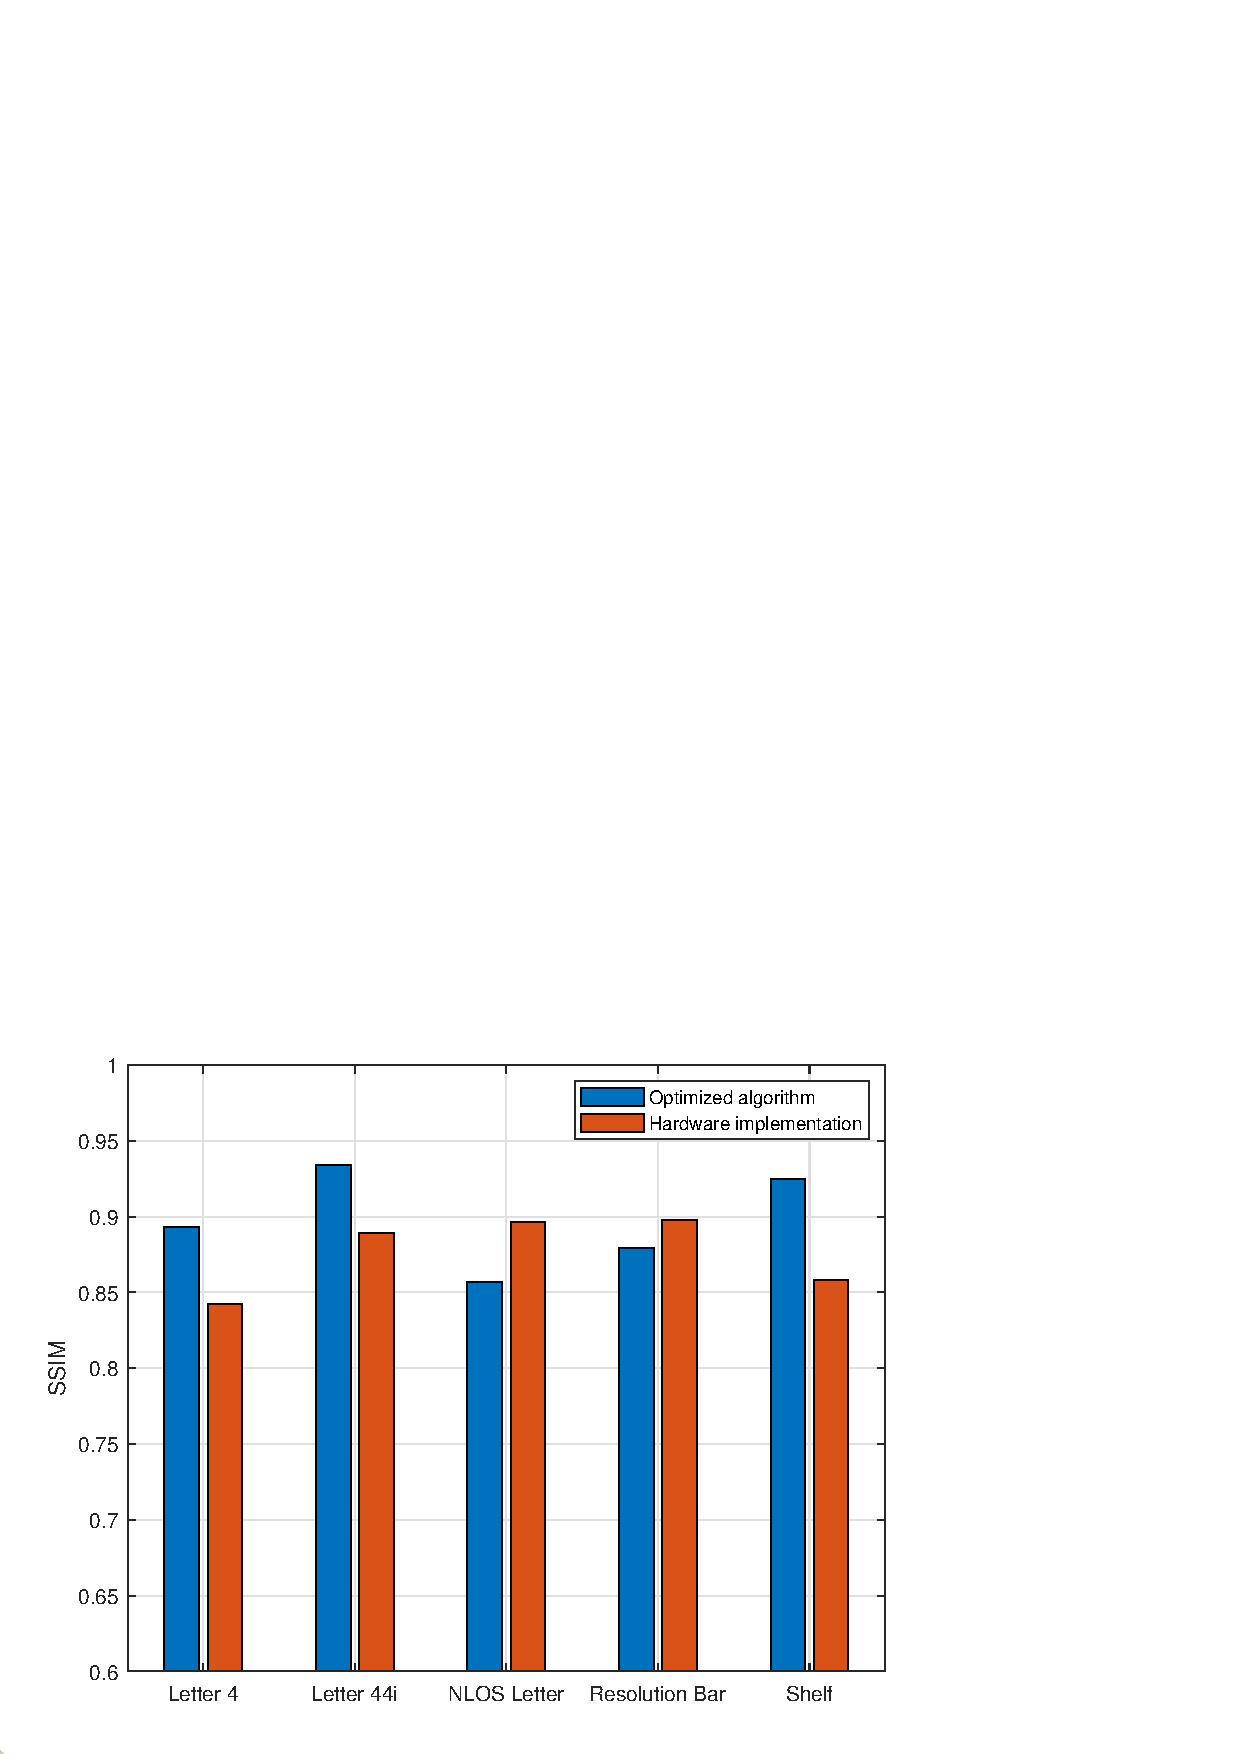
\includegraphics[width=\textwidth]{figure/hw_opt_ori_res_comp.pdf}
    \bicaption{用优化后算法的重构结果、硬件实现的重构结果,比较原始算法的结果,所得的SSIM值。}{SSIM of the results generated by the optimized RSD algorithm and hardware implementation, comparing to the original results.}
    \label{fig:ssim}
\end{figure}

\begin{figure}[!tb]
  \centering
  \includegraphics[width=\textwidth]{figure/diffmap/ssim_letter4.pdf}
  \bicaption{Letter 4的SSIM差异图。}{Letter 4 differential map.}
  \label{fig:ssim_l4}
\end{figure}

\begin{figure}[!tb]
  \centering
  \includegraphics[width=\textwidth]{figure/diffmap/ssim_letter44i.pdf}
  \bicaption{Letter 44i的SSIM差异图。}{Letter 44i differential map.}
  \label{fig:ssim_l44i}
\end{figure}

\begin{figure}[!tb]
  \centering
  \includegraphics[width=\textwidth]{figure/diffmap/ssim_nlos.pdf}
  \bicaption{Letter NLOS的SSIM差异图。}{Letter NLOS differential map.}
  \label{fig:ssim_nlos}
\end{figure}

\begin{figure}[!tb]
  \centering
  \includegraphics[width=\textwidth]{figure/diffmap/ssim_resolutionbar.pdf}
  \bicaption{Resolution Bar的SSIM差异图。}{Resolution Bar differential map.}
  \label{fig:ssim_resolutionbar}
\end{figure}

\begin{figure}[!tb]
  \centering
  \includegraphics[width=\textwidth]{figure/diffmap/ssim_shelf.pdf}
  \bicaption{Shelf的SSIM差异图。}{Shelf differential map.}
  \label{fig:ssim_shelf}
\end{figure}

值得一提的是,对于在真实实验环境下采集的NLOS成像数据,目前并没有定量的比较方法来衡量重构结果和真实的隐藏场景之间的相似程度,即重构的效果到底如何基本还是依靠人眼判断。并且,不同的NLOS成像算法之间也没有公认的基准,这是因为所有的NLOS成像算法所重构出的场景都远不如LOS成像的真实。因此,除非使用的NLOS数据来自计算机渲染的场景,其他的针对真实场景的NLOS成像算法都是依靠视觉的比较来衡量重构的效果。这也是衡量基于RSD的NLOS成像算法重构效果所用的方法\citep{Liu,Liu2019}。

\section{FPGA实现结果}

在CPU上运行的原始的基于RSD的NLOS重构算法使用的数据格式是未经量化的浮点数。然而,对于硬件加速器的设计而言,浮点数运算操作耗费的资源太多。因此合理地使用FPGA上的硬件资源,我们需要将算法所需的所有数据包括中间结果量化为定点数格式。表\ref{tab:quant}总结了本文所提出的加速器设计中使用的量化策略。

\begin{table}[!t]
    \centering
    \bicaption{加速器的量化策略}{Quantization Scheme of Accelerator}
    \label{tab:quant}
    \resizebox{.7\textwidth}{!}{
    \begin{tabular}{@{}ccccc@{}}
    \toprule
                 & 整数位宽 & 小数位宽 & 总位宽 & 数据类型           \\ \midrule
    Input signal & 14            & -6             & 8         & Complex   \\ \midrule
    \textit{Wave}         & 8             & 8              & 16        & Real      \\ \midrule
    \textit{Distance}     & 8             & 8              & 16        & Real      \\ \midrule
    \textit{Timeshift}    & -4            & 20             & 16        & Complex   \\ \midrule
    Coefficients & -5            & 21             & 16        & Complex   \\ \midrule
    RSD kernel   & 0             & 16             & 16        & Complex   \\ \midrule
    FFT out      & 10            & 2              & 12        & Complex   \\ \midrule
    MAC result   & 10            & 8              & 18        & Complex   \\ \midrule
    IFFT out     & 6             & 12             & 18        & Complex   \\ \bottomrule
    \end{tabular}}
\end{table}

图\ref{fig:nlossys}中所示的是本文演示的NLOS成像加速器的系统框图。整个系统由一个NLOSI Core,一个RSD核数据驱动模块(Kernel Driver),一个NLOS数据驱动模块(Image Driver),以及一个HDMI接口模块组成。RSD核驱动模块包括一些只读存储模块(ROM)存储了重构RSD核所需的单位环形脉冲函数以及对应的线性组合系数,并驱动一个AXI总线。NLOSI Core挂载在AXI总线上,以接收相应的数据。NLOS数据驱动模块则存储了待输入的瞬态图像数据并通过Stream数据通道(一种遵守valid-ready握手协议的数据通道)将数据送入NLOSI Core。这里使用的NLOS数据均采集自真实环境的瞬态图像,也被\citet{Liu,Liu2019}用于演示其NLOS成像算法,且这些数据均以开源。HDMI接口模块将重构结果包装为符合HDMI协议的视频流格式,并将该视频信号通过一个FMC接口传送至HDMI子卡上。以上所述的包含在加速器系统里的四个模块均实现在Intel Stratix 10 SoC FPGA上,如图\ref{fig:testsys}所示。HDMI子卡插在FPGA板卡的FMC接口上,并通过HDMI线连接至外部的一台显示器上,将经过处理转换的重构结果显示在显示器上。图\ref{fig:testsys}展示了整个NLOS成像加速器系统在显示器上显示的重构结果。
\begin{table}[!t]
    \centering
    \bicaption{性能比较}{Performance Comparison}
    \label{tab:perf_comp}
    \resizebox{\textwidth}{!}{
    \begin{tabular}{@{}cccc@{}}
    \toprule
               & 原始RSD算法\citep{Liu} & 优化后RSD算法 & 硬件加速器 \\ \midrule
    Platform   & AMD R7 4800HS               & AMD R7 4800HS                  & Stratix 10 \\ \midrule
    Clock (MHz) & N/A                         & N/A                            & 50         \\ \midrule
    Time (one frame)      & 2.34s                       & 0.83s                          & 39.5ms     \\ \midrule
    Speed (FPS) & 0.42                        & 1.2                            & 25.31      \\  \bottomrule
    % Power (W)   & N/A                         & N/A                            & 10         \\ \bottomrule
    \end{tabular}}
\end{table}

\begin{figure}[!tb]
  \centering
  \includegraphics[width=\textwidth]{figure/system.pdf}
  \bicaption{演示的NLOS系统框图。}{Block diagram of the demonstration system.}
  \label{fig:nlossys}
\end{figure}

\begin{figure}[!tb]
  \centering
  \includegraphics[width=\textwidth]{figure/testsys_demo.pdf}
  \bicaption{实现在FPGA上的系统的照片。}{Photo of the NLOS imaging accelerator implemented on FPGA.}
  \label{fig:testsys}
\end{figure}

截至目前,本文作者尚未发现其他公开发表的基于RSD算法的NLOS成像硬件加速器设计相关的文献,包括以FPGA或者ASIC方式实现。因此在成像性能上,我们只能与原始的基于RSD的NLOS重构算法和优化后的算法的软件实现进行比较。这里NLOS成像系统参数的设置和\citet{Liu}一致,其中$N_D=51, N_\Omega=69, N_R=68, K=128$。两个算法都运行在MATLAB R2020a上,电脑配置为AMD R7 4800HS CPU以及16GB内存。表\ref{tab:perf_comp}总结了性能比较的结果。很明显,以CPU为平台运行基于RSD的NLOS成像算法,无论是原始的版本还是优化后的版本,都无法满足实时NLOS成像的要求。而在FPGA上实现的NLOS成像加速平台,可以在一个相对较低的运行频率——50 MHz的时钟频率——下也能满足25FPS的要求。当然,我们可以通过提高时钟频率或者增加加速器的资源预算,来获得一个更高的成像帧率。
\begin{table}[!t]
    \centering
    \bicaption{资源利用率}{Resource Utilization}
    \label{tab:util}
    \setlength{\tabcolsep}{5mm}{
    \begin{tabular}{@{}ccccc@{}}
    \toprule
    资源    & ALM    & FF      & BRAM  & DSP  \\ \midrule
    已用的        & 618672 & 269462  & 4777  & 1413 \\ \midrule
    可用的   & 933120 & 1866240 & 11721 & 5760 \\ \midrule
    利用率 & 66\%   & 14\%    & 41\%  & 25\% \\ \bottomrule
    \end{tabular}}
\end{table}
\begin{figure}[!tb]
    \centering
    \includegraphics[width=.75\textwidth]{figure/util_break.pdf}
    \bicaption{资源利用率饼图。}{Breakdown of the resource utilizations.}
    \label{fig:util_break}
\end{figure}

演示的NLOS成像系统的硬件资源利用率如表\ref{tab:util}所示,对应的饼图则展示在\ref{fig:util_break}。从中可以看到,模块RSD GenCore和FFT2D Core占据了硬件资源的主要部分(约90\%)。

\chapter{总结与展望}

在这篇文章里,我们

\textcolor{red}{TODO.}

\makebiblio

\appendix
\chapter{可能的附录}
% 本章中的测试材料,数学公式部分来自 \textsf{ucasthesis} 附录 B\footnote{\url{https://github.com/mohuangrui/ucasthesis/blob/master/Tex/Appendix.tex}},生僻字部分来自《生僻字大全(按部首分类)》\footnote{\url{http://xh.5156edu.com/page/z4745m2559j18770.html}}。

\section{附录1}
% \providecommand{\Vector}[1]{\ensuremath{\symbf{ #1 }}}
% \providecommand{\Tensor}[1]{\ensuremath{\symbfup{ #1 }}}
% \begin{equation}
%   \begin{cases}
%       \frac{\partial \rho}{\partial t} + \nabla\cdot(\rho\Vector{V}) = 0 \\
%       \frac{\partial (\rho\Vector{V})}{\partial t} + \nabla\cdot(\rho\Vector{V}\Vector{V}) = \nabla\cdot\Tensor{\sigma} \\
%       \frac{\partial (\rho E)}{\partial t} + \nabla\cdot(\rho E\Vector{V}) = \nabla\cdot(k\nabla T) + \nabla\cdot(\Tensor{\sigma}\cdot\Vector{V})
%   \end{cases}
% \end{equation}
% \begin{equation}
%   \frac{\partial }{\partial t}\int\limits_{\Omega} u \, \symup{d}\Omega + \int\limits_{S} \Vector{n}\cdot(u\Vector{V}) \, \symup{d}S = \dot{\phi}
% \end{equation}
% \begin{equation*}
%   \begin{split}
%       \symcal{L} \{f\}(s) &= \int _{0^{-}}^{\infty} f(t) e^{-st} \, \symup{d}t, \ 
%       \symscr{L} \{f\}(s) = \int _{0^{-}}^{\infty} f(t) e^{-st} \, \symup{d}t\\
%       \symcal{F} {\bigl (} f(x+x_{0}) {\bigr )} &= \symcal{F} {\bigl (} f(x) {\bigr )} e^{2\pi i\xi x_{0}}, \ 
%       \symscr{F} {\bigl (} f(x+x_{0}) {\bigr )} = \symscr{F} {\bigl (} f(x) {\bigr )} e^{2\pi i\xi x_{0}}
%   \end{split}
% \end{equation*}

% \begin{center}
% \begin{tabular}{*{4}{l}}
%   \toprule
%   Ordinary math& $A,F,L,2,3,5,\sigma$& \verb|\symup|& $\symup{A,F,L,2,3,5,\sigma}$ \\
%   \verb|\symbf|& $\symbf{A,F,L,2,3,5,\sigma}$& \verb|\symit|& $\symit{A,F,L,2,3,5,\sigma}$ \\
%   \verb|\symsf|& $\symsf{A,F,L,2,3,5,\sigma}$& \verb|\symtt|& $\symtt{A,F,L,2,3,5,\sigma}$ \\
%   \verb|\symfrak|& $\symfrak{A,F,L,2,3,5,\sigma}$& \verb|\symbb|& $\symbb{A,F,L,2,3,5,\sigma}$ \\
%   \verb|\symcal|& $\symcal{A,F,L,2,3,5,\sigma}$& \verb|\symscr|& $\symscr{A,F,L,2,3,5,\sigma}$ \\
%   \bottomrule
% \end{tabular}
% \end{center}

\section{附录2} 
% {\songti 叧叨叭叱叴叵叺叻叼叽叾卟叿吀吁吂吅吆吇吋吒吔吖吘吙吚吜吡吢吣吤吥吧吩吪吭吮吰吱吲呐吷吺吽呁呃呄呅呇呉呋呋呌呍呎呏呐呒呓呔呕呗呙呚呛呜呝呞呟呠呡呢呣呤呥呦呧周呩呪呫呬呭呮呯呰呱呲呴呶呵呷呸呹呺呻呾呿咀咁咂咃咄咅咇咈咉咊咋咍咎咐咑咓咔咕咖咗咘咙咚咛咜咝咞咟咠咡咢咣咤咥咦咧咨咩咪咫咬咭咮咯咰咲咳咴咵咶啕咹咺咻呙咽咾咿哂哃哅哆哇哈哊哋哌哎哏哐哑哒哓哔哕哖哗哘哙哚哛哜哝哞哟哠咔哣哤哦哧哩哪哫哬哯哰唝哵哶哷哸哹哻哼哽哾哿唀唁唂唃呗唅唆唈唉唊唋唌唍唎唏唑唒唓唔唣唖唗唘唙吣唛唜唝唞唟唠唡唢唣唤唥唦唧唨唩唪唫唬唭唯唰唲唳唴唵唶唷念唹唺唻唼唽唾唿啀啁啃啄啅啇啈啉啋啌啍啎问啐啑啒启啔啕啖啖啘啙啚啛啜啝哑启啠啡唡衔啥啦啧啨啩啪啫啬啭啮啯啰啱啲啳啴啵啶啷啹啺啻啼啽啾啿喀喁喂喃善喅喆喇喈喉喊喋喌喍喎喏喐喑喒喓喔喕喖喗喙喛喞喟喠喡喢喣喤喥喦喨喩喯喭喯喰喱哟喳喴喵営喷喸喹喺喼喽喾喿嗀嗁嗂嗃嗄嗅呛啬嗈嗉唝嗋嗌嗍吗嗏嗐嗑嗒嗓嗕嗖嗗嗘嗙呜嗛嗜嗝嗞嗟嗠嗡嗢嗧嗨唢嗪嗫嗬嗭嗮嗰嗱嗲嗳嗴嗵哔嗷嗸嗹嗺嗻嗼嗽嗾嗿嘀嘁嘂嘃嘄嘅嘅嘇嘈嘉嘊嘋嘌喽嘎嘏嘐嘑嘒嘓呕嘕啧嘘嘙嘚嘛唛嘝嘞嘞嘟嘠嘡嘢嘣嘤嘥嘦嘧嘨哗嘪嘫嘬嘭唠啸囍嘴哓嘶嘷呒嘹嘺嘻嘼啴嘾嘿噀噂噃噄咴噆噇噈噉噊噋噌噍噎噏噐噑噒嘘噔噕噖噗噘噙噚噛噜咝噞噟哒噡噢噣噤哝哕噧噩噪噫噬噭噮嗳噰噱哙噳喷噵噶噷吨噺噻噼噽噾噿咛嚁嚂嚃嚄嚅嚆吓嚈嚉嚊嚋哜嚍嚎嚏尝嚑嚒嚓嚔噜嚖嚗嚘啮嚚嚛嚜嚝嚞嚟嚠嚡嚢嚣嚤呖嚧咙嚩咙嚧嚪嚫嚬嚭嚯嚰嚱亸喾嚵嘤嚷嚸嚹嚺嚻嚼嚽嚾嚿啭嗫嚣囃囄冁囆囇呓囊囋囍囎囏囐嘱囒啮囔囕囖}

% {\heiti 圠圡圢圤圥圦圧圩圪圫圬圮圯地圱圲圳圴圵圶圷圸圹圻圼埢鴪址坁坂坃坄坅坆坈坉坊坋坌坍坒坓坔坕坖坘坙坜坞坢坣坥坧坨坩坪坫坬坭坮坯垧坱坲坳坴坶坸坹坺坻坼坽坾坿垀垁垃垅垆垇垈垉垊垌垍垎垏垐垑垓垔垕垖垗垘垙垚垛垜垝垞垟垠垡垤垥垧垨垩垪垫垬垭垮垯垰垱垲垲垳垴埯垶垷垸垹垺垺垻垼垽垾垽垿埀埁埂埃埄埅埆埇埈埉埊埋埌埍城埏埐埑埒埓埔埕埖埗埘埙埚埛野埝埞域埠垭埢埣埤埥埦埧埨埩埪埫埬埭埮埯埰埱埲埳埴埵埶执埸培基埻崎埽埾埿堀堁堃堄坚堆堇堈堉垩堋堌堍堎堏堐堑堒堓堔堕垴堗堘堙堚堛堜埚堞堟堠堢堣堥堦堧堨堩堫堬堭堮尧堰报堲堳场堶堷堸堹堺堻堼堽堾堼堾碱塀塁塂塃塄塅塇塆塈塉块茔塌塍塎垲塐塑埘塓塕塖涂塘塙冢塛塜塝塟塠墘塣墘塥塦塧塨塩塪填塬塭塮塯塰塱塲塳塴尘塶塷塸堑塺塻塼塽塾塿墀墁墂墄墅墆墇墈墉垫墋墌墍墎墏墐墒墒墓墔墕墖墘墖墚墛坠墝增墠墡墢墣墤墥墦墧墨墩墪樽墬墭堕墯墰墱墲坟墴墵垯墷墸墹墺墙墼墽垦墿壀壁壂壃壄壅壆坛壈壉壊垱壌壍埙壏壐壑壒压壔壕壖壗垒圹垆壛壜壝垄壠壡坜壣壤壥壦壧壨坝塆圭}

% {\kaishu 奵奺奻奼奾奿妀妁妅妉妊妋妌妍妎妏妐妑妔妕妗妘妚妛妜妟妠妡妢妤妦妧妩妫妭妮妯妰妱妲妴妵妶妷妸妺妼妽妿姀姁姂姃姄姅姆姇姈姉姊姌姗姎姏姒姕姖姘姙姛姝姞姟姠姡姢姣姤姥奸姧姨姩姫姬姭姮姯姰姱姲姳姴姵姶姷姸姹姺姻姼姽姾娀威娂娅娆娈娉娊娋娌娍娎娏娐娑娒娓娔娕娖娗娙娚娱娜娝娞娟娠娡娢娣娤娥娦娧娨娩娪娫娬娭娮娯娰娱娲娳娴娵娷娸娹娺娻娽娾娿婀娄婂婃婄婅婇婈婋婌婍婎婏婐婑婒婓婔婕婖婗婘婙婛婜婝婞婟婠婡婢婣婤婥妇婧婨婩婪婫娅婮婯婰婱婲婳婵婷婸婹婺婻婼婽婾婿媀媁媂媄媃媅媪媈媉媊媋媌媍媎媏媐媑媒媓媔媕媖媗媘媙媚媛媜媝媜媞媟媠媡媢媣媤媥媦媨媩媪媫媬媭妫媰媱媲媳媴媵媶媷媸媹媺媻媪媾嫀嫃嫄嫅嫆嫇嫈嫉嫊袅嫌嫍嫎嫏嫐嫑嫒嫓嫔嫕嫖妪嫘嫙嫚嫛嫜嫝嫞嫟嫠嫡嫢嫣嫤嫥嫦嫧嫨嫧嫩嫪嫫嫬嫭嫮嫯嫰嫱嫲嫳嫴嫳妩嫶嫷嫸嫹嫺娴嫼嫽嫾婳妫嬁嬂嬃嬄嬅嬆嬇娆嬉嬊娇嬍嬎嬏嬐嬑嬒嬓嬔嬕嬖嬗嬘嫱嬚嬛嬜嬞嬟嬠嫒嬢嬣嬥嬦嬧嬨嬩嫔嬫嬬奶嬬嬮嬯婴嬱嬲嬳嬴嬵嬶嬷婶嬹嬺嬻嬼嬽嬾嬿孀孁孂娘孄孅孆孇孆孈孉孊娈孋孊孍孎孏嫫婿媚}

% {\fangsong 敳屮屰屲屳屴屵屶屷屸屹屺屻屼屽屾屿岃岄岅岆岇岈岉岊岋岌岍岎岏岐岑岒岓岔岕岖岘岙岚岜岝岞岟岠岗岢岣岤岥岦岧岨岪岫岬岮岯岰岲岴岵岶岷岹岺岻岼岽岾岿峀峁峂峃峄峅峆峇峈峉峊峋峌峍峎峏峐峑峒峓崓峖峗峘峚峙峛峜峝峞峟峠峢峣峤峥峦峧峨峩峪峬峫峭峮峯峱峲峳岘峵峷峸峹峺峼峾峿崀崁崂崃崄崅崆崇崈崉崊崋崌崃崎崏崐崒崓崔崕崖崘崚崛崜崝崞崟岽崡峥崣崤崥崦崧崨崩崪崫崬崭崮崯崰崱崲嵛崴崵崶崷崸崹崺崻崼崽崾崿嵀嵁嵂嵃嵄嵅嵆嵇嵈嵉嵊嵋嵌嵍嵎嵏岚嵑岩嵓嵔嵕嵖嵗嵘嵙嵚嵛嵜嵝嵞嵟嵠嵡嵢嵣嵤嵥嵦嵧嵨嵩嵪嵫嵬嵭嵮嵯嵰嵱嵲嵳嵴嵵嵶嵷嵸嵹嵺嵻嵼嵽嵾嵿嶀嵝嶂嶃崭嶅嶆岖嶈嶉嶊嶋嶌嶍嶎嶏嶐嶑嶒嶓嵚嶕嶖嶘嶙嶚嶛嶜嶝嶞嶟峤嶡峣嶣嶤嶥嶦峄峃嶩嶪嶫嶬嶭崄嶯嶰嶱嶲嶳岙嶵嶶嶷嵘嶹岭嶻屿岳帋巀巁巂巃巄巅巆巇巈巉巊岿巌巍巎巏巐巑峦巓巅巕岩巗巘巙巚}

\backmatter
\begin{acknowledgement}
% \shtthesis{} 派生于中国科学院大学论文模板 \textsf{ucasthesis}\footnote{\url{https://github.com/mohuangrui/ucasthesis},使用 GPLv3 许可证分发。};v0.2.0 开发过程中参考了清华大学论文模板 \textsf{thuthesis}\footnote{\url{https://www.ctan.org/pkg/thuthesis},使用 LPPL-1.3c 许可证分发。},特别是 \verb|\thusetup| 命令的设计和实现;v0.3.0 及后续版本开发过程中参考了复旦大学论文模板 \textsf{fduthesis}\footnote{\url{https://www.ctan.org/pkg/fduthesis},使用 LPPL-1.3c 许可证分发。},以及其超链接配色方案。这些项目中流淌的智慧,以及项目作者们的专业态度和共享精神使得 \shtthesis{} 的开发及完善成为可能。
致谢部分。
\end{acknowledgement}

\ifgraduate
\begin{resume}
  廖正鹏,上海科技大学信息学院2019级硕士研究生,导师娄鑫。
\end{resume}

\begin{publications}
  FPGA Accelerator for Real-Time Non-Line-of-Sight Imaging
\end{publications}

\begin{publications*}
  FPGA Accelerator for Real-Time Non-Line-of-Sight Imaging
\end{publications*}

% \begin{patents}
%   专利申请或授权记录…… (非匿名环境)
% \end{patents}

% \begin{patents*}
%   专利申请或授权记录…… (匿名环境)
% \end{patents*}

% \begin{projects}
%   个人参与的科研项目、获奖情况…… (仅非匿名环境显示)
% \end{projects}
\fi

\end{document}
